% ******************************* PhD Thesis Template **************************
% Please have a look at the README.md file for info on how to use the template

\documentclass[a4paper,12pt,times,numbered,print,index,custombib]{Classes/PhDThesisPSnPDF}

% ******************************************************************************
% ******************************* Class Options ********************************
% *********************** See README for more details **************************
% ******************************************************************************

% `a4paper'(The University of Cambridge PhD thesis guidelines recommends a page
% size a4 - default option) or `a5paper': A5 Paper size is also allowed as per
% the Cambridge University Engineering Deparment guidelines for PhD thesis
%
% `11pt' or `12pt'(default): Font Size 10pt is NOT recommended by the University
% guidelines
%
% `oneside' or `twoside'(default): Printing double side (twoside) or single
% side.
%
% `print': Use `print' for print version with appropriate margins and page
% layout. Leaving the options field blank will activate Online version.
%
% `index': For index at the end of the thesis
%
% `draftclassic': For draft mode without loading any images (same as draft in book)
%
% `draft': Special draft mode with line numbers, images, and water mark with
% timestamp and custom text. Position of the text can also be modified.
%
% `abstract': To generate only the title page and abstract page with
% dissertation title and name, to submit to the Student Registry
%
% `chapter`: This option enables only the specified chapter and it's references
%  Useful for review and corrections.
%
% ************************* Custom Page Margins ********************************
%
% `custommargin`: Use `custommargin' in options to activate custom page margins,
% which can be defined in the preamble.tex. Custom margin will override
% print/online margin setup.
%
% *********************** Choosing the Fonts in Class Options ******************
%
% `times' : Times font with math support. (The Cambridge University guidelines
% recommend using times)
%
% `fourier': Utopia Font with Fourier Math font (Font has to be installed)
%            It's a free font.
%
% `customfont': Use `customfont' option in the document class and load the
% package in the preamble.tex
%
% default or leave empty: `Latin Modern' font will be loaded.
%
% ********************** Choosing the Bibliography style ***********************
%
% `authoryear': For author-year citation eg., Krishna (2013)
%
% `numbered': (Default Option) For numbered and sorted citation e.g., [1,5,2]
%
% `custombib': Define your own bibliography style in the `preamble.tex' file.
%              `\RequirePackage[square, sort, numbers, authoryear]{natbib}'.
%              This can be also used to load biblatex instead of natbib
%              (See Preamble)
%
% **************************** Choosing the Page Style *************************
%
% `default (leave empty)': For Page Numbers in Header (Left Even, Right Odd) and
% Chapter Name in Header (Right Even) and Section Name (Left Odd). Blank Footer.
%
% `PageStyleI': Chapter Name next & Page Number on Even Side (Left Even).
% Section Name & Page Number in Header on Odd Side (Right Odd). Footer is empty.
%
% `PageStyleII': Chapter Name on Even Side (Left Even) in Header. Section Number
% and Section Name in Header on Odd Side (Right Odd). Page numbering in footer


% ********************************** Preamble **********************************
% Preamble: Contains packages and user-defined commands and settings
\usepackage{titlesec}
\usepackage{pgfplots}
\pgfplotsset{width=9cm,compat=1.9}
\usepackage[utf8]{inputenc} 
\usepackage{graphicx}
%\usepackage[spanish]{babel}
\usepackage{xcolor}
\usepackage{listings}
\usepackage{csquotes}
\usepackage{dirtree}
\usepackage{minted}

\lstset{
	basicstyle={\scriptsize\ttfamily},
	tabsize=2
}

% ******************************************************************************
% ****************************** Custom Margin *********************************

% Add `custommargin' in the document class options to use this section
% Set {innerside margin / outerside margin / topmargin / bottom margin}  and
% other page dimensions
\ifsetCustomMargin
  \RequirePackage[left=37mm,right=30mm,top=35mm,bottom=30mm]{geometry}
  \setFancyHdr % To apply fancy header after geometry package is loaded
\fi

% Add spaces between paragraphs
%\setlength{\parskip}{0.5em}
% Ragged bottom avoids extra whitespaces between paragraphs
\raggedbottom
% To remove the excess top spacing for enumeration, list and description
%\usepackage{enumitem}
%\setlist[enumerate,itemize,description]{topsep=0em}

% *****************************************************************************
% ******************* Fonts (like different typewriter fonts etc.)*************

% Add `customfont' in the document class option to use this section

\ifsetCustomFont
  % Set your custom font here and use `customfont' in options. Leave empty to
  % load computer modern font (default LaTeX font).
  %\RequirePackage{helvet}

  % For use with XeLaTeX
  %  \setmainfont[
  %    Path              = ./libertine/opentype/,
  %    Extension         = .otf,
  %    UprightFont = LinLibertine_R,
  %    BoldFont = LinLibertine_RZ, % Linux Libertine O Regular Semibold
  %    ItalicFont = LinLibertine_RI,
  %    BoldItalicFont = LinLibertine_RZI, % Linux Libertine O Regular Semibold Italic
  %  ]
  %  {libertine}
  %  % load font from system font
  %  \newfontfamily\libertinesystemfont{Linux Libertine O}
\fi

% *****************************************************************************
% **************************** Custom Packages ********************************

% ************************* Algorithms and Pseudocode **************************

%\usepackage{algpseudocode}


% ********************Captions and Hyperreferencing / URL **********************

% Captions: This makes captions of figures use a boldfaced small font.
%\RequirePackage[small,bf]{caption}

\RequirePackage[labelsep=space,tableposition=top]{caption}
\renewcommand{\figurename}{Fig.} %to support older versions of captions.sty

% ########################## Renombrado ##########################
\renewcommand{\appendixpagename}{Apendice}

% changes the default name `Bibliography` -> `References'
\renewcommand{\bibname}{Bibliografía}

\def\acknowledgementsname{acknowledgements}
\renewcommand{\acknowledgementsname}{Agradecimientos}

\renewcommand{\chaptername}{Capítulo}

\renewcommand{\contentsname}{Tabla de Contenidos}
\renewcommand{\listfigurename}{Tabla de Figuras}
\renewcommand{\listtablename}{Tabla de Cuadros}

\renewcommand{\appendixtocname}{Lista de apendices}
\renewcommand{\appendixname}{Apendice}

% *************************** Graphics and figures *****************************

%\usepackage{rotating}
%\usepackage{wrapfig}

% Uncomment the following two lines to force Latex to place the figure.
% Use [H] when including graphics. Note 'H' instead of 'h'
%\usepackage{float}
%\restylefloat{figure}

% Subcaption package is also available in the sty folder you can use that by
% uncommenting the following line
% This is for people stuck with older versions of texlive
%\usepackage{sty/caption/subcaption}
\usepackage{subcaption}

% ********************************** Tables ************************************
\usepackage{booktabs} % For professional looking tables
\usepackage{multirow}

%\usepackage{multicol}
%\usepackage{longtable}
%\usepackage{tabularx}


% *********************************** SI Units *********************************
\usepackage{siunitx} % use this package module for SI units


% ******************************* Line Spacing *********************************

% Choose linespacing as appropriate. Default is one-half line spacing as per the
% University guidelines

% \doublespacing
% \onehalfspacing
% \singlespacing


% ************************ Formatting / Footnote *******************************

% Don't break enumeration (etc.) across pages in an ugly manner (default 10000)
%\clubpenalty=500
%\widowpenalty=500

%\usepackage[perpage]{footmisc} %Range of footnote options


% *****************************************************************************
% *************************** Bibliography  and References ********************

%\usepackage{cleveref} %Referencing without need to explicitly state fig /table

% Add `custombib' in the document class option to use this section
\ifuseCustomBib
   \RequirePackage[square, sort, numbers, authoryear]{natbib} % CustomBib

% If you would like to use biblatex for your reference management, as opposed to the default `natbibpackage` pass the option `custombib` in the document class. Comment out the previous line to make sure you don't load the natbib package. Uncomment the following lines and specify the location of references.bib file

%\RequirePackage[backend=biber, style=numeric-comp, citestyle=numeric, sorting=nty, natbib=true]{biblatex}
\bibliography{References/references} %Location of references.bib only for biblatex

\fi

% changes the default name `Bibliography` -> `References'
\renewcommand{\bibname}{References}


% ******************************** Roman Pages *********************************
% The romanpages environment set the page numbering to lowercase roman one
% for the contents and figures lists. It also resets
% page-numbering for the remainder of the dissertation (arabic, starting at 1).

\newenvironment{romanpages}{
  \setcounter{page}{1}
  \renewcommand{\thepage}{\roman{page}}}
{\newpage\renewcommand{\thepage}{\arabic{page}}}


% ******************************************************************************
% ************************* User Defined Commands ******************************
% ******************************************************************************

% *********** To change the name of Table of Contents / LOF and LOT ************

%\renewcommand{\contentsname}{My Table of Contents}
%\renewcommand{\listfigurename}{My List of Figures}
%\renewcommand{\listtablename}{My List of Tables}


% ********************** TOC depth and numbering depth *************************

\setcounter{secnumdepth}{4}
\setcounter{tocdepth}{2}


% ******************************* Nomenclature *********************************

% To change the name of the Nomenclature section, uncomment the following line

%\renewcommand{\nomname}{Symbols}


% ********************************* Appendix ***********************************

% The default value of both \appendixtocname and \appendixpagename is `Appendices'. These names can all be changed via:

%\renewcommand{\appendixtocname}{List of appendices}
%\renewcommand{\appendixname}{Appndx}

% *********************** Configure Draft Mode **********************************

% Uncomment to disable figures in `draftmode'
%\setkeys{Gin}{draft=true}  % set draft to false to enable figures in `draft'

% These options are active only during the draft mode
% Default text is "Draft"
%\SetDraftText{DRAFT}

% Default Watermark location is top. Location (top/bottom)
%\SetDraftWMPosition{bottom}

% Draft Version - default is v1.0
%\SetDraftVersion{v1.1}

% Draft Text grayscale value (should be between 0-black and 1-white)
% Default value is 0.75
%\SetDraftGrayScale{0.8}


% ******************************** Todo Notes **********************************
%% Uncomment the following lines to have todonotes.

%\ifsetDraft
%	\usepackage[colorinlistoftodos]{todonotes}
%	\newcommand{\mynote}[1]{\todo[author=kks32,size=\small,inline,color=green!40]{#1}}
%\else
%	\newcommand{\mynote}[1]{}
%	\newcommand{\listoftodos}{}
%\fi

% Example todo: \mynote{Hey! I have a note}


% ************************ Thesis Information & Meta-data **********************
% Thesis title and author information, refernce file for biblatex
% ************************ Thesis Information & Meta-data **********************
%% The title of the thesis
\title{Escalabilidad de Redes Definidas por Software en la Red Académica}
%\texorpdfstring is used for PDF metadata. Usage:
%\texorpdfstring{LaTeX_Version}{PDF Version (non-latex)} eg.,
%\texorpdfstring{$sigma$}{sigma}

%% Subtitle (Optional)
\subtitle{Proyecto de grado}

%% The full name of the author
\author{ \fontsize{12pt}{12pt}\selectfont {\normalfont \textbf{Santiago Vidal} } \\ \vspace{1cm} Supervisores: \\ {\normalfont Dr. Eduardo Grampín \\ MSc. Martín Giachino \\}}
%% Department (eg. Department of Engineering, Maths, Physics)
\dept{\fontsize{12pt}{12pt}\selectfont Instituto de Computación}

%% University and Crest
\university{Facultad de Ingeniería, Universidad de la República}
% Crest minimum should be 30mm.
\crest{
	
\includegraphics[width=0.185\textwidth]{Udelar} 
	\hspace{3cm}
	
\includegraphics[width=0.25\textwidth]{fing}
	\vspace{1cm}
}
%% Use this crest, if you are using the college crest
%% Crest long miminum should be 65mm
%\crest{\includegraphics[width=0.45\textwidth]{University_Crest_Long}}

%% College shield [optional] 
% Crest minimum should be 30mm.
%\collegeshield{\includegraphics[width=0.2\textwidth]{CollegeShields/Kings}}


%% Supervisor (optional)
%% Supervisor Role (optional) - Supervisor (default) or advisor
%\supervisorrole{Advisor: }

%% Advisor (optional)
%\advisor{Prof. Malcolm Bolton}
%% Advisor Role (optional) - Advisor (default) or leave empty
%\advisorrole{Advisor: }


%% You can redefine the submission text:
% Default as per the University guidelines:
% ``This dissertation is submitted for the degree of''
\renewcommand{\submissiontext}{}


%% College affiliation (optional)
%\college{\fontsize{11pt}{12pt}\selectfont Facultad de Ingeniería, Universidad de la República}

%% Submission date
% Default is set as {\monthname[\the\month]\space\the\year}
\degreedate{Junio 2016} 


% ***************************** Abstract Separate ******************************
% To printout only the titlepage and the abstract with the PhD title and the
% author name for submission to the Student Registry, use the `abstract' option in
% the document class.

\ifdefineAbstract
 \pagestyle{empty}
 \includeonly{Declaration/declaration, Abstract/abstract}
\fi

% ***************************** Chapter Mode ***********************************
% The chapter mode allows user to only print particular chapters with references
% Title, Contents, Frontmatter are disabled by default
% Useful option to review a particular chapter or to send it to supervisior.
% To use choose `chapter' option in the document class

\ifdefineChapter
 \includeonly{Chapter3/chapter3}
\fi

% ******************************** Front Matter ********************************
\begin{document}

\frontmatter

\begin{titlepage}
  \maketitle
\end{titlepage}


%% ******************************* Thesis Dedidcation ********************************

\begin{dedication} 

I would like to dedicate this thesis to my loving parents \dots

\end{dedication}


%% ************************** Thesis Acknowledgements **************************

\begin{acknowledgements}      


And I would like to acknowledge ...


\end{acknowledgements}

%% ************************** Thesis Abstract *****************************
% Use `abstract' as an option in the document class to print only the titlepage and the abstract.
\begin{abstract2}
Las Redes Definidas por Software (SDN) es un paradigma de red que plantea desacoplar el plano de datos y el plano de control, además de estandarizar el modo en que se debe manipular a los dispositivos de red. Esto significa una gran mejora con respecto a las redes tradicionales, ya que permite a los administradores e investigadores desarrollar nuevos servicios y protocolos de forma más ágil y rápida, sin tener que preocuparse por aspectos comerciales de tecnologías propietarias ni de la complejidad de los protocolos distribuidos. Sin embargo, no es realista plantear un cambio repentino de un modelo a otro. Por lo tanto, es importante plantear trabajos que puedan aprovechar SDN y al mismo tiempo puedan convivir, e incluso aprovechar las tecnologías legadas. Un ejemplo de esto es RAUFlow, una propuesta de implementación desarrollada en 2015 para la nueva Red Académica Uruguaya. RAUFlow utiliza el enfoque SDN y al mismo tiempo ciertos aspectos de los protocolos legados para proveer redes privadas virtuales como servicio.

En este proyecto se continúa el trabajo sobre la arquitectura RAUFlow, teniendo como principal enfoque su escalabilidad, de cara a un posible despliegue en la nueva Red Académica Uruguaya. Para ello se construye una herramienta de virtualización que permite emular la arquitectura RAUFlow, y se utiliza la misma para hacer pruebas que no serían posibles con un prototipo físico. Además de ofrecer una herramienta con capacidades funcionales que no se han observado en ninguna otra herramienta disponible, se contribuye al campo con un estudio a fondo de las aplicaciones del modelo SDN, así como de sus tecnologías de virtualización disponibles.

\textbf{Palabras clave:} Redes de Computadoras, SDN, OpenFlow, Open vSwitch, Emuladores de red, Mininet
\end{abstract2}


% *********************** Adding TOC and List of Figures ***********************

\tableofcontents

\listoffigures

\listoftables

% \printnomenclature[space] space can be set as 2em between symbol and description
%\printnomenclature[3em]

\printnomenclature

% ******************************** Main Matter *********************************
\mainmatter

\chapter{Introducción}
La Red Académica Uruguaya (RAU) es un emprendimiento de la Universidad de la República que ya lleva 28 años, y es administrado por el Servicio Central de Informática Universitario (SeCIU). Al igual que las redes académicas de muchos otros países, tiene como objetivo proveer a docentes e investigadores una infraestructura aislada de las redes comerciales, que les ofrezca altas velocidades para diversas aplicaciones de enseñanza e investigación. La RAU actualmente consta de 64 nodos y brinda servicios a 31 instituciones, abarcando un total aproximado de 8.000 docentes, 4.000 técnicos y 100.000 estudiantes\footnote{Cifras obtenidas del informe del proyecto RRAP}.

En la actualidad se está trabajando en renovar la RAU con una nueva infraestructura que permita proveer más y mejores servicios. Este esfuerzo se denominó RAU2. Los principales objetivos de esta renovación son: 1) extender y mejorar la calidad del servicio, y 2) implementar servicios e infraestructuras que maximicen la sinergia entre las instituciones. Para esto, se plantean tres áreas principales de trabajo: re-diseñar la topología de la red y aumentar el ancho de banda, mejorar la controlabilidad de la red, y desarrollar una plataforma integrada y global para los servicios académicos.

En 2015 culminó un proyecto llamado Routers Reconfigurables de Altas Prestaciones (RRAP) \cite{proyecto-rrap} que consistió en la construcción de un prototipo para la RAU2. Este prototipo propone una arquitectura de red denominada RAUFlow, y está basada en un concepto llamado Redes Definidas por Software (SDN por sus siglas en inglés). SDN es un paradigma de red que ha tomado fuerza en los últimos años, que plantea desacoplar el plano de control (donde se determina qué hacer con los paquetes de datos) del plano de datos (donde se toman las acciones sobre los paquetes). Propone una infraestructura enfocada en otorgar, de forma más económica y eficiente, un mayor control a los operadores de red para adaptar y optimizar sus redes para los servicios y capacidades que necesitan proveer.

A pesar de la fuerza que han ganado las redes definidas por software en el último tiempo, están lejos de ser el estándar, y las redes legadas aún son muy utilizadas en la actualidad. Por esta razón es necesario estudiar soluciones que aprovechen las ventajas que ofrece SDN, y al mismo tiempo puedan coexistir con las redes legadas y beneficiarse de las mismas. RAUFlow es una propuesta que sigue ese mismo principio de redes híbridas, y es la base sobre la que se construye este trabajo.
% **************************** Define Graphics Path **************************
\graphicspath{{Chapter1/Figs/}}

\section{Proyecto RRAP}
El prototipo para la RAU2 construido por el proyecto RRAP \cite{proyecto-rrap} está compuesto 4 routers y una arquitectura para el control de la red basada en SDN, llamada RAUFlow. Cada dispositivo se denomina RAUSwitch y tiene la capacidad de funcionar en modo SDN y en modo tradicional como router IP. Los aspectos técnicos, tanto de RAUFlow como de RAUSwitch, se analizarán más adelante.
El prototipo fue verificado con una serie de pruebas funcionales que comprueban la validez del enfoque y que se proveen correctamente los servicios de red que fueron implementados.
Sin embargo, debido a las limitaciones físicas del prototipo, el enfoque propuesto aún no ha sido validado con pruebas de escala que aseguren que el mismo podría ser adoptado para una infraestructura con una dimensión y carga como la que tiene la RAU.

\section{Objetivos}
El objetivo principal de este trabajo es estudiar la escalabilidad de la arquitectura RAUFlow mediante simulaciones con grandes cantidades de nodos. Dada la ausencia de trabajos relacionados a la virtualización de redes híbridas que soporten SDN y los protocolos IP tradicionales, previamente es necesario un estudio a fondo de las tecnologías de virtualización disponibles y un posterior trabajo de construcción de la plataforma deseada.

\section{Resultados esperados}
Se espera que este trabajo produzca los siguientes resultados:
\begin{itemize}
	\item El estado del arte en lo que refiere a la implementación de aplicaciones en SDN, así como las herramientas de virtualización disponibles, prestando especial atención a aquellas que pueden ser aplicables al enfoque híbrido SDN/Legacy y al mismo tiempo sean escalables.
	\item Una herramienta que permita virtualizar la arquitectura RAUFlow, y que sea razonablemente escalable. Es importante considerar dicha herramienta como un resultado que pueda mantenerse útil incluso afuera del contexto de RAUFlow, como herramienta de investigación autocontenida.
	\item Diseñar y llevar a cabo una serie de pruebas de escala sobre RAUFlow que detecten posibles errores, y permitan hacer un análisis sobre su escalabilidad.
\end{itemize}

\section{Estructura del documento}
La estructura de lo que resta de este documento se explica a continuación. En el capítulo 2 se muestran los resultados de la investigación del estado del arte. En el mismo se explican algunos conceptos claves para entender este trabajo, entre ellos los aspectos técnicos de RAUFlow y RAUSwitch. Luego se estudia lo investigado con respecto a las aplicaciones de SDN y las herramientas de virtualización disponibles. En el capítulo 3 se presentan los requerimientos, diseño, implementación y problemas encontrados para el entorno virtual construido. En el capítulo 4 se presentan las pruebas de escala realizadas y un análisis de los resultados que arrojan. Por último, en el capítulo 5 se presentan las conclusiones de la realización de este trabajo y posibles líneas de trabajo futuro.

Además, se agrega un capítulo con la bibliografía utilizada y un apéndice con el manual de usuario para el entorno virtual.


\chapter{Estado del arte}

% **************************** Define Graphics Path **************************
\graphicspath{{Chapter2/Figs/}}

\section{Software Defined Networking}
Aspectos generales
%https://www.necam.com/docs/?id=2709888a-ecfd-4157-8849-1d18144a6dda

%http://www.iaria.org/conferences2014/filesICNS14/InfoSys%202014%20Control%20Plane%20Scalability%20in%20SDN-%20%20v1.2.pdf

%http://arxiv.org/pdf/1408.6760.pdf

\section{OpenFlow}
Aspectos generales
%http://article.sciencepublishinggroup.com/pdf/10.11648.j.ajsea.20140306.12.pdf

%http://www.spirent.com/~/media/White%20Papers/Broadband/PAB/OpenFlow_Performance_Testing_WhitePaper.pdf

\section{Open vSwitch}
%http://openvswitch.org/pipermail/discuss/2012-February/006447.html

%http://openvswitch.org/support/dist-docs/ovs-vswitchd.8.txt

%http://benpfaff.org/papers/ovs.pdf

%http://networkheresy.com/2014/11/13/accelerating-open-vswitch-to-ludicrous-speed/

%http://bluesy.wang/notes/2014/09/14/flow-caching-for-high-entropy-packet-fields/

%http://yuba.stanford.edu/~nickm/papers/flow-caching.pdf

%http://wangcong.org/2012/10/20/an-overview-of-openvswitch-implementation/

%https://www.google.com/url?sa=t&rct=j&q=&esrc=s&source=web&cd=1&ved=0ahUKEwixpuyBieLLAhUCdR4KHVV7CKgQFggfMAA&url=https%3A%2F%2Fnsrc.org%2Fworkshops%2F2014%2Fnznog-sdn%2Fraw-attachment%2Fwiki%2FAgenda%2FOpenVSwitch.pdf&usg=AFQjCNFg9VULvEmHMXQAsuTOE6XLH6WbzQ&bvm=bv.117868183,d.dmo&cad=rja

%http://openvswitch.org/slides/OpenStack-131107.pdf

%http://openvswitch.org/slides/openvswitch.en-2.pdf

%https://www.google.com/url?sa=t&rct=j&q=&esrc=s&source=web&cd=3&ved=0ahUKEwjP95D9ieLLAhVIpB4KHUKeCzYQFggoMAI&url=http%3A%2F%2Fopenvswitch.org%2Fsupport%2Fovscon2014%2F17%2F1530-ovsconf2014_chadnorgan.pptx&usg=AFQjCNEmnrXDB0psj5oXvoAzVYr8F5sLtQ&cad=rja

%https://www.google.com/url?sa=t&rct=j&q=&esrc=s&source=web&cd=1&cad=rja&uact=8&ved=0ahUKEwjZvdvaiuLLAhWF1h4KHfYrCKoQFggiMAA&url=http%3A%2F%2Fopenvswitch.org%2Fsupport%2Fovscon2014%2F18%2F1600-ovs_perf.pptx&usg=AFQjCNGGTT0rHmENeZ2ZcoRfWNFJ__hBLw

\section{Multiprotocol Label Switching (MPLS)}
Conceptos básicos

\section{Red Privada Virtual (VPN)}
Conceptos básicos

\section{Aplicaciones de SDN}
El paradigma SDN, por definición, está basado en el software. Esto implica que el rango de aplicaciones o modos de uso que se le puede dar al paradigma es enorme. En esta sección se estudiarán algunas aplicaciones existentes sobre SDN, haciendo foco en la implementación de redes privadas virtuales, debido a que es el servicio que provee RAUFlow.
\subsection{Implementación de VPNs}
El desarrollo de redes privadas virtuales (VPN) es un tema relativamente común en SDN, ya que es un servicio de gran utilidad. A continuación se estudiarán algunas implementaciones existentes de VPN sobre SDN. \\ \\
\textbf{Proyecto CoCo} \\
CoCo \cite{coco-paper} es un proyecto que estudia el desarrollo de un servicio de VPN multipunto enfocado hacia investigadores, para permitirles intercambiar información de modo confiable y seguro. Uno de sus principales enfoques es la facilidad de uso, lo cual es una ventaja frente a las implementaciones tradicionales (no SDN) de este servicio. Sólo requiere que el administrador haga una configuración inicial de la red, y luego los usuarios finales pueden crear, modificar y  eliminar VPNs a demanda mediante un portal web. \\ \\
La arquitectura de CoCo consiste de múltiples dominios, y cada dominio tiene una infraestructura basada en OpenFlow. Los switches OpenFlow de cada dominio son manejados por un controlador OpenDaylight, llamado agente CoCo. Cada agente CoCo se encarga de administrar el plano de datos de su dominio (esto es: reglas de forwarding, descubrimiento de topología, etc) y de conectarse con los otros agentes, es decir, con los otros dominios. Esto último lo hace mediante el protocolo BGP.

%https://blog.surf.nl/en/coco-an-exploration-of-software-defined-networking/
%http://www.nec.com/en/global/techrep/journal/g13/n02/pdf/130212.pdf
%http://yuba.stanford.edu/~nickm/papers/ofc11-saurav-mpls.pdf
\subsection{Otras aplicaciones}
Monitorización de red
Load balancing / QoS
Prevención de DoS
%http://ieeexplore.ieee.org.proxy.timbo.org.uy:443/stamp/stamp.jsp?tp=&arnumber=6567024
%http://ieeexplore.ieee.org.proxy.timbo.org.uy:443/stamp/stamp.jsp?tp=&arnumber=6983147
Implementación de Servicios de red

\section{Simuladores y emuladores}
\subsection{DOT} %es distribuido, asi que no aplicaria mucho, pero esta bueno, asi que capaz que si
\subsection{Estinet} %si
\subsection{fs-sdn} %si
\subsection{Mininet} %si
Mininet es un emulador de redes SDN que permite emular hosts, switches, controladores y enlaces. Utiliza virtualización basada en procesos para ejecutar múltiples instancias (hasta 4096) de hosts y switches en un unico kernel de sistema operativo. También utiliza una capacidad de Linux denominada \textit{network namespace} que permite crear "interfaces de red virtuales", y de esta manera dotar a los nodos con sus propias interfaces, tablas de ruteo y tablas ARP. Lo que en realidad hace Mininet es utilizar la arquitectura \textit{Linux container}, que tiene la capacidad de proveer virtualización completa, pero de un modo reducido ya que no requiere de todas sus capacidades. Mininet también utiliza \textit{virtual ethernet (veth)} para crear los enlaces virtuales entre los nodos.

Mencionar MaxiNet (está en las referencias)
Capaz mencionar Mininet-HiFi (buscar en el survey) %http://tiny-tera.stanford.edu/~nickm/papers/p253.pdf
Capaz mencionar Mininet CE (buscar en el survey)
Capaz mencionar SDN Cloud DC (buscar en el survey)
\subsection{NS-3} %si
%The popular network simulator NS-3 also offers an OpenFlow simulation model [8]. However, this model in its current version does not model the OpenFlow controller as an external entity. Therefore, it is not possible to quantify the effects of the control channel or simulate multiple switches connected to a single OpenFlow controller.
%tambien lo de openflow 1.3
\subsection{OFNet} %si, aunque parece estar muy en desarrollo todavia

\subsection{Otras herramientas}
\begin{itemize}
	\item Flowsim
	\item STS
	\item Omnet++
	\item Opencontrail
	\item CORE
\end{itemize}
%\subsection{Flowsim} %es mas bien didactico asi que no
%\subsection{STS} %es orientado a troubleshooting asi que no
%\subsection{Omnet++} %puede ser, pero no se puede usar rauflow, asi que capaz que no
%\subsection{Opencontrail} %creo que no, es un controlador asi que pareceria  que no
%\subsection{CORE} %usa ovs, asi que se podria mencionar aca

%\section{Simuladores/emuladores no SDN}
%\subsection{Unified Networking Lab} %no
%\subsection{VNX y VNUML} %no
%\subsection{OpenStack} %no
%\subsection{OPNET} %no
%\subsection{Psimulator2} %no
%\subsection{Shadow} %no
%\subsection{MLN} %no
%\subsection{Netkit}
%\subsection{NetSim} %no
%\subsection{GNS3} %no
%\subsection{LINE} %no
%\subsection{Marionnet} %no
%\subsection{Cloonix} %no

\section{Herramientas para pruebas de estrés y benchmarking}
Existen múltiples herramientas de testing aplicables en el paradigma SDN. De ellas se puede destacar un grupo, que no tienen como objetivo verificar aspectos funcionales, sino que apuntan a algo mucho más específico: las pruebas de estrés y el benchmarking. Ayudan a los administradores de red e investigadores a conocer los niveles de rendimiento de los cuales sus dispositivos y redes son capaces. Asimismo, pueden ser elementos de investigación útiles en el contexto de la nueva Red Académica, ya que podrían utilizarse, por ejemplo, para validar ciertos aspectos de rendimiento de los RAUSwitch.

En esta sección se estudiarán algunos ejemplos de estas herramientas, agrupándolas en dos grupos, de acuerdo a la entidad que intentan probar: switches y controladores. Para mantener la relevancia con el contexto de este trabajo, se limitará a herramientas enfocadas a OpenFlow.

\subsection{Testing de switches}
El testing y benchmarking de switches OpenFlow tiene como objetivo analizar cuál es el nivel máximo de rendimiento que puede alcanzar un switch. Esto por lo general se logra simulando las condiciones de una red que está bajo mucha carga, y sometiendo al switch a dichas condiciones, monitoreando su comportamiento. A continuación se listan algunas herramientas que hacen esto:
\begin{itemize}
	\item \textbf{OFLOPS} \cite{oflops} (OpenFlow Operations Per Second) es un framework open source para el testing y benchmarking de switches OpenFlow, tanto físicos como virtuales. Está desarrollado en el lenguaje C, y utiliza librerías de manipulación de paquetes para emular un controlador OpenFlow y tráfico de uso. Fue diseñado con un enfoque multi-thread para aprovechar las arquitecturas multi-core y así aumentar la potencia de la plataforma. Consiste de cinco threads paralelos, cada uno cumpliendo una función específica: 1) generación de paquetes, 2) captura de paquetes, 3) administración del canal de control (mensajes OpenFlow), 4) administración de un canal SNMP para hacer consultas asíncronas, y 5) un manejador de tiempo. Todo esto lo ofrece mediante una API, permitiendo a los usuarios crear sus propios módulos para escribir pruebas que se adapten a su realidad.
	\item \textbf{Spirent OpenFlow Controller Emulation} \cite{spirent-controller-emulation} es una herramienta desarrollada por la empresa Spirent\footnote{http://spirent.com/} que, igual que OFLOPS, tiene como propósito el testing y benchmarking de switches OpenFlow. Puede emular un controlador OpenFlow, definir millones de flujos y aplicar patrones de tráfico a esos flujos, y de ese modo medir el rendimiento, disponibilidad, seguridad y escalabilidad del switch. Entre sus funcionalidades, se destaca que puede probar todos los aspectos de OpenFlow 1.3, y que puede trabajar con switches híbridos. Estos dos puntos lo hacen una valiosa herramienta para el testing de la arquitectura RAUFlow.
\end{itemize}

\subsection{Testing de controladores}
Similar al caso de los switches, las pruebas de estrés sobre controladores OpenFlow consisten en someterlos a condiciones de mucha carga y estudiar determinadas métricas de su comportamiento. En general los principales aspectos que se buscan estudiar son 1) la cantidad de sesiones paralelas con switches OpenFlow que puede mantener el controlador y 2) el ritmo de mensajes packet\_in que puede manejar. No sólo es útil conocer esos umbrales, sino que también es muy valioso saber cual es el comportamiento esperado si se exceden dichos umbrales. Al ser RAUFlow un controlador de estilo proactivo, el aspecto número dos no es relevante aquí, ya que la red no genera paquetes de tipo packet\_in. A continuación se listan algunas de las herramientas disponibles:
\begin{itemize}
	\item \textbf{Cbench} \cite{cbench} es una herramienta para benchmarking de controladores, y es parte del proyecto OFLOPS. Su funcionamiento es muy simple: el usuario indica una cantidad \textit{n} de switches, la herramienta crea \textit{n} sesiones OpenFlow paralelas con el controlador, y luego comienza a enviar mensajes de tipo packet\_in y mide el tiempo que demora el controlador en responder a esos mensajes.
	\item \textbf{Spirent OpenFlow Switch Emulation} \cite{spirent-switch-emulation} es la propuesta de Spirent para el stress-testing de controladores OpenFlow. Igual que Cbench, en esencia consiste en emular múltiples switches y generar mensajes de tipo packet\_in. Sin embargo, es una solución un poco más sofisticada que Cbench, ya que permite trabajar con múltiples topologias y protocolos como ARP y LLDP.
\end{itemize}



\chapter{Entorno virtual}

% **************************** Define Graphics Path **************************
\graphicspath{{Chapter3/Figs/}}

Uno de los principales objetivos de este trabajo es realizar pruebas funcionales y de escala sobre la arquitectura del prototipo. Es de interés generar distintas realidades, y así detectar puntos de falla o variables clave en la performance de la arquitectura. Para modelar las distintas realidades se puede utilizar dos parámetros: topología y servicios. Es importante poder aplicar topologias complejas y relativamente grandes a la arquitectura, así como grandes cantidades de servicios, y de esta forma encontrar posibles problemas con la arquitectura, y su respectiva solución. Dado que no es realista hacer este tipo de pruebas con un prototipo físico, por temas económicos y prácticos, se observa la necesidad de un entorno virtual capaz de simular las características del prototipo. Es importante remarcar que también tendría un gran valor como herramienta de investigación, para trabajar sobre la arquitectura de RAUFlow pero también para futuros estudios sobre esquemas híbridos SDN/Legacy. \\
En este capítulo se estudian los requerimientos que debe cumplir este entorno, las herramientas estudiadas, y los detalles de diseño e implementación de la solución construida. También se explican los principales problemas o dificultades encontradas para lograr un correcto funcionamiento, así como el desarrollo de un módulo que permite cargar topologias automáticamente desde archivos con formato GraphML.

\section{Requerimientos del entorno virtual}
El primer paso en la construcción del entorno virtual es analizar cómo debería comportarse. Se podría hacer este análisis en dos partes separadas. En primer lugar, se deben cumplir los aspectos funcionales de la arquitectura de RAUFlow. No es un requerimiento que se utilicen las mismas herramientas, porque puede que sea tecnológicamente imposible, pero es deseable que así sea. Cuanto más similar sea el entorno a la arquitectura, más relevantes serán las pruebas que se lleven a cabo. Otra ventaja es que se pueden reutilizar recursos, como por ejemplo, archivos de configuración. En el segundo grupo, se consideran los requerimientos inherentes a un entorno de simulación como el que se pretende. \\
El primer grupo de requerimientos se detalla a continuación.

\begin{itemize}
	\item Se debe poder simular múltiples RAUSwitch virtuales, y los mismos deben tener las mismas capacidades funcionales que sus pares físicos. A partir de esto, se desprenden los siguientes sub-requerimientos.
	\begin{itemize}
		\item Deben poder utilizar el protocolo de enrutamiento OSPF. Esto es necesario ya que la base de datos topológica de RAUFlow se construye a partir de la base de datos local de OSPF (Link-State Database).  Es deseable que lo hagan mediante el software de enrutamiento Quagga.
		\item Resulta trivial que los RAUSwitch virtuales soporten OpenFlow, ya que es el cimiento de RAUFlow. Pero es importante que soporten la versión 1.3. Esto se debe a que la implementación de las VPNs depende de que los nodos tengan soporte para MPLS, y OpenFlow ofrece esta funcionalidad a partir de la versión 1.3 (???). Es muy deseable que lo hagan mediante Open vSwitch, ya que es lo que utilizan los RAUSwitch físicos.
		\item En la arquitectura de RAUFlow se usan agentes SNMP para que los RAUSwitch envíen información que no es soportada por el protocolo OpenFlow acerca de sus interfaces. Como requerimiento para este entorno, es importante que los nodos puedan enviar esa información de algún modo, pero no es necesario que sea a través de SNMP, ya que no es una parte vital de la arquitectura.
	\end{itemize}
	\item Se debe poder simular múltiples hosts, ya que son los agentes que se conectan a la red y utilizan la misma para enviarse datos entre sí. De esta forma se corrobora que el funcionamiento de la red es el correcto.
	\item La aplicación RAUFlow debe ejecutarse y comunicarse correctamente con los RAUSwitch. Esto también implica que el controlador Ryu debe ser soportado por el entorno.
\end{itemize}

El segundo grupo de requerimientos es más genérico, ya que son los que surgen para casi cualquier entorno de simulación de redes.

\begin{itemize} 
	\item Facilidad de configuración. Es importante que el entorno pueda generar distintas topologias y escenarios sin demasiado esfuerzo de configuración.
	\item Escalabilidad. Dado que uno de los objetivos es realizar pruebas de escala, el entorno debería ofrecer buena escalabilidad en la cantidad de nodos que puede simular. Esto se traduce a que una computadora promedio de uso personal pueda levantar algunas decenas de nodos virtuales como mínimo.
\end{itemize}

\section{Elección de la herramienta}
%No es realista construirlo de cero, asi que se necesita una herramienta.
%Esta basado en Open vSwitch
%Provee ejemplos sobre como usar Quagga
%Escalable
%Api Python para fácil configuración de topologias


\section{Diseño e implementación del entorno}
El entorno está construido alrededor de Mininet, y se podría pensar como una extensión de la misma. \textit{Out of the box}, Mininet ya cumple la mayoría de los requerimientos estudiados anteriormente. Está diseñada para ser escalable, ya que usa containers reducidos, tiene soporte para OpenFlow 1.3 mediante OpenVSwitch, y gracias a su API en Python es muy fácil de configurar. El aspecto en el que falla es en el soporte para Quagga. Dado que Mininet es una herramienta de prototipado para SDN puro, no está pensado para un esquema híbrido como el que se propone. Los switches compatibles con OpenVSwitch que ofrece no pueden tener su propio network namespace, por lo tanto, no pueden tener su propia tabla de ruteo ni interfaces de red aisladas, así que no es posible que utilicen Quagga.

Por otro lado, los hosts de Mininet sí tienen su propio network namespace, y gracias a su capacidad de tener sus propios procesos y directorios, podemos ejecutar una instancia de Quagga y OpenVSwitch para cada host. De esta forma es posible crear un router como el requerido por la arquitectura. Esta extensión de las funcionalidades de los hosts es posible ya que Mininet está programado con orientación a objetos y permite al usuario crear subclases propias de las clases que vienen por defecto. En la figura \ref{fig:clases_entorno} se puede ver la estructura de clases del entorno construido. En las siguientes secciones se procederá a estudiar cada una de ellas.

\begin{figure}[t]
	\caption{Diagrama de clases del entorno.}
	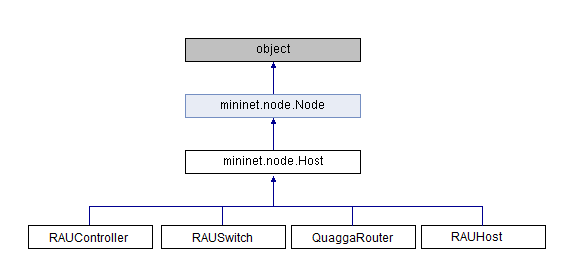
\includegraphics[scale=0.65]{clases_entorno}
	\centering
	\label{fig:clases_entorno}
\end{figure}

\subsection{RAUController}
En el uso típico de Mininet, la comunicación entre el controlador y el switch se da a través de la interfaz de loopback. Esto es así porque los switches no tienen su propio namespace. Para lograr dicha comunicación, no hace falta un objeto en Mininet que represente el controlador, ya que ejecutar la aplicación en el sistema operativo base ya habilita al switch a comunicarse con ella a través de la interfaz de loopback. Esta situación cambia en este diseño, porque los switches pasan a tener su propio network namespace. Esto lleva a la necesidad de crear un host virtual, que ejecute la aplicación de RAUFlow y se comunique con los switches a través de enlaces virtuales. Para satisfacer esta necesidad se usa la clase RAUController.

\subsection{RAUSwitch}
La clase RAUSwitch es el núcleo del entorno de simulación. Es un Host extendido de tal forma para que, gracias a la funcionalidad de directorios privados, ejecute su propia instancia de Quagga y OpenVSwitch. Cada RAUSwitch tiene los siguientes directorios privados: /var/log/, /var/log/quagga, /var/run, /var/run/quagga, /var/run/openvswitch. Cada RAUSwitch también usa un directorio bajo /tmp, para almacenar sus archivos de configuración.\\ \\

OpenVSwitch básicamente consiste de 2 demonios (ovs-vswitchd y ovsdb-server) que ejecutan en el user-space, y un módulo en el kernel que actúa como cache para los flujos recientes. Utiliza el protocolo 'netlink' para comunicar el user-space con el módulo en el kernel. Poder tomar decisiones sobre los paquetes a nivel del kernel, sin tener que pasar por el user-space, explica en gran medida el buen nivel de performance que ofrece OpenVSwitch. Sin embargo, tener múltiples módulos de kernel ejecutando en el mismo sistema operativo puede crear comportamientos impredecibles e incorrectos, ya que no está previsto para trabajar de esa forma.\\
Afortunadamente, OpenVSwitch puede ejecutarse completamente en modo user-space, es decir, sin soporte del módulo del kernel. Esto implica que podemos ejecutar tantas instancias de OpenVSwitch como queramos, pero la performance va a ser significativamente peor. Esto no es una desventaja muy seria, ya que el objetivo del entorno no es ser performante al procesar paquetes. Cabe aclarar que en este modo OpenVSwitch continúa haciendo cacheo de flujos, pero ahora lo hace en el user-space.

\begin{figure}[t]
	\caption{Arquitectura de OpenVSwitch.}
	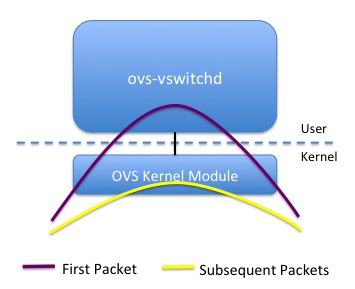
\includegraphics[scale=0.65]{ovs_dataplane}
	\centering
	\label{fig:ovs_dataplane}
\end{figure}

\subsection{QuaggaRouter}
Es una clase similar al RAUSwitch pero sin Open vSwitch, es decir, sólo usa Quagga. Apunta a representar el router CE que utilizaría una subred para conectarse a la red. Está conectado a un RAUSwitch de borde.

\subsection{RAUHost}
Representa a los hosts que serán clientes de la red. Con este propósito, se podría utilizar directamente la clase Host de Mininet, pero se construye esta clase auxiliar para evitar determinadas configuraciones manuales, como por ejemplo, el \textit{default gateway}.

\subsection{Sustitución del agente SNMP}
Como se explicó en el capítulo (X), RAUFlow usa un agente SNMP en cada switch para hacer disponible al controlador, información acerca de sus interfaces de red que no puede enviar a través de OpenFlow. Específicamente, los datos que se envían a través de SNMP para cada interfaz de red son dirección IP, dirección MAC y nombre de interfaz. Para lograr esto en el entorno virtual se debe crear una instancia de agente SNMP por cada RAUSwitch virtual que se ejecuta, y se las debe configurar de tal forma para que cada una sólo devuelva la información de su nodo virtual. \\
Si bien es posible, se observa que lograr esto es relativamente complejo, debido que se aleja mucho del uso tradicional de SNMP. A esto se suma el hecho de que si bien es necesario que esa información llegue al controlador de alguna forma, no es estrictamente necesario que sea mediante SNMP. Por lo tanto, se concluye que la información que RAUFlow envía al controlador a través de SNMP, sea enviada de otra forma en el entorno virtual.

La alternativa que se construye está basada en Open vSwitch. Mediante el comando 'ovs-vsctl list bridge', se pueden ver las distintas propiedades del switch, como el identificador de datapath, estado, etc. Entre esas propiedades, existe un campo llamado 'other\_config', al que se le pueden agregar un número de configuraciones adicionales. Entonces, se utiliza ese campo para almacenar una propiedad llamada 'ports\_info' que almacenará la información sobre todas las interfaces del nodo. Esta propiedad no tendrá significado para Open vSwitch, por lo tanto quedará intacta. El valor que almacenará la propiedad debe ser de tipo String, y probablemente almacene la información de múltiples interfaces de red, así que se debe crear un formato para esa información. Por ejemplo, si tenemos un switch con la siguiente información:
\begin{lstlisting}
Interfaz de red 1:
	Nombre: eth1
	Direccion IP: 10.0.0.1
	Direccion MAC: 00:00:00:00:00:01
Interfaz de red 2:
	Nombre: eth2
	Direccion IP: 10.0.0.2
	Direccion MAC: 00:00:00:00:00:02
\end{lstlisting}
El valor de ports\_info sería el siguiente:
\begin{lstlisting}
eth1_10.0.0.1_00:00:00:00:00:01/eth2_10.0.0.2_00:00:00:00:00:02
\end{lstlisting}

Como se puede ver, el formato indica que se usa el carácter '/' para separar la información de cada interfaz, y el carácter '\_' para dividir los campos de información de cada interfaz. Este formato no es el único posible, se puede utilizar cualquier otro siempre y cuando use los caracteres permitidos por Open vSwitch.

Después de configurar el campo ports\_info, cada instancia de Open vSwitch almacena la información de las interfaces de su respectivo nodo virtual. Sin embargo, esta información todavía no es accesible desde afuera del nodo. Para lograr que Open vSwitch pueda enviar esta información por la red, se utiliza un comando llamado 'set-manager'. Con él, se le puede indicar a Open vSwitch que escuche en un determinado puerto (típicamente el puerto TCP 6640) para que pueda ser gestionado de forma remota. Por lo tanto, si el controlador desea saber los datos de las interfaces de un determinado switch, alcanza con que le envíe el comando 'ovs-vsctl list bridge' a través de la red y parsear la respuesta para extraer los datos de interés.

Como se explicó anteriormente, esta alternativa se construye para evitar la adaptación de SNMP al entorno virtual. Sin embargo, se considera que es una buena solución al problema de los datos de las interfaces. En primer lugar, la arquitectura se simplifica, ya que elimina la necesidad de SNMP. Esta solución utiliza aspectos de Open vSwitch, que ya está integrada a la arquitectura, por lo que no agrega mucha complejidad. En segundo lugar, eliminar la necesidad de que cada nodo ejecute un agente SNMP ayuda a la performance de los mismos. Por estas razones, se sugiere esta solución como aporte a RAUFlow.

\section{Módulo de carga automática - GraphML Loader}
Como se explica en el Apéndice 1, cada topología se debe configurar en un script Python usando la API del entorno. Este proceso puede ser tedioso, especialmente si se trata de una topología grande. Todos los nodos se deben inicializar con los parámetros que requieren, también se deben crear los enlaces entre ellos, y cualquier problema de coherencia en los datos puede resultar en un funcionamiento inadecuado de la topología.

Tomando como base \cite{auto-mininet}, se desarrolló un módulo llamado \textbf{GraphML Loader}. Su propósito es facilitar la tarea de configurar topologias nuevas. GraphML es un formato de archivo que sirve para detallar grafos (sus nodos, enlaces, etc), y está basado en XML. Este formato es usado, por ejemplo, en el dataset de Topology Zoo \cite{topology-zoo} para detallar las topologias. El propósito de este módulo es recibir como entrada un archivo de tipo graphml y producir como salida un script Python que configura la topología que se corresponde con el grafo de entrada. El módulo se encarga no sólo de crear una topología que se adapte al grafo, sino que también de asignar automáticamente las direcciones IP de cada nodo, indicar qué nodos son de borde y cuales no, entre muchas otras cosas. Este módulo aporta una gran mejora a la usabilidad del entorno virtual, ya que si el usuario dispone de un archivo de tipo graphml, puede tener una topología lista para usarse en pocos segundos. En caso que se desee hacer una modificación a dicha topología, alcanza con hacerla en el script que produjo el módulo. En el Apéndice 2 se explica más detalladamente como funciona este componente.


\section{Problemas y errores encontrados}
Como resultado de las pruebas funcionales básicas que se efectuaron sobre el entorno (que son detalladas en la sección 4.1.1) se detectaron determinados problemas que fueron necesarios estudiar. Esta sección explicará en que consiste cada problema, estudiando sus síntomas, su explicación, y en caso de que exista una, su solución. Como se verá, algunos de ellos se manifestarían en un despliegue real de la arquitectura, y otros son a causa del uso de un entorno virtual, y por lo tanto no se deberían tener en cuenta en un despliegue real.

\subsection{Errores en el código de RAUFlow}
Se descubrió que existían determinados errores (o "bugs") en el código de RAUFlow. Como son errores en el código del controlador, es importante remarcar que estos errores sin lugar a dudas se manifestarían en una red real. \\ \\
\textbf{Error en flujos de servicio con más de un salto} \\
\begin{figure}[t]
	\caption{Escenario donde los flujos están mal configurados. Muestra la topología de la red y los flujos de interés para cada nodo.}
	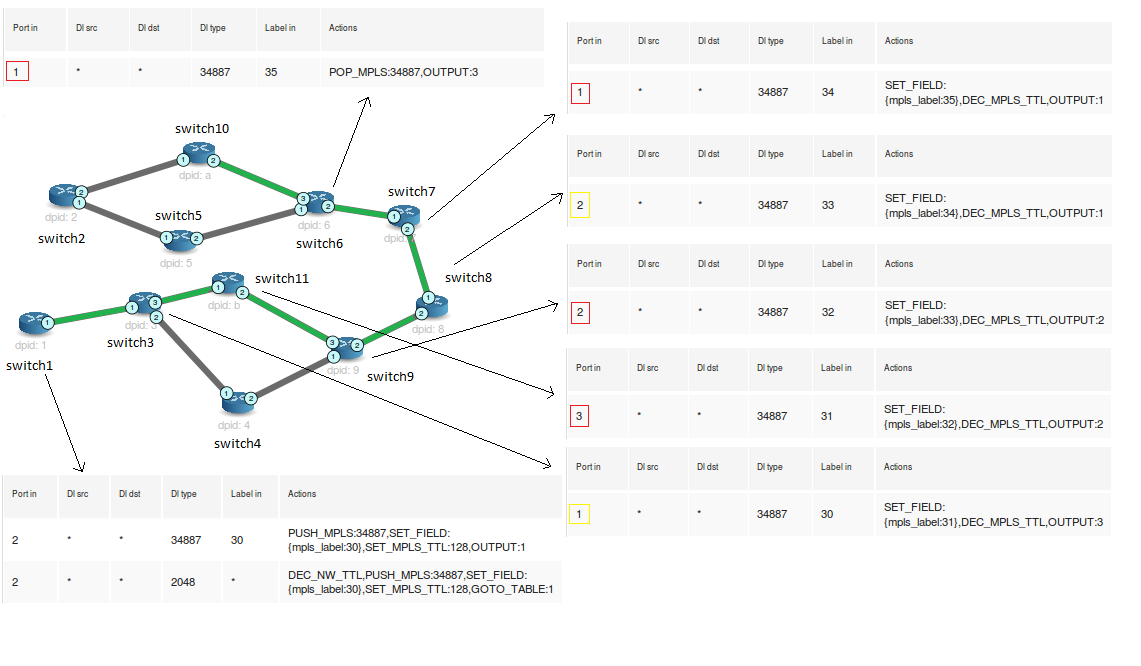
\includegraphics[scale=0.5]{flujos_incorrectos}
	\centering
	\label{fig:flujos_incorrectos}
\end{figure}
Se observó que cuando se trataba de crear un servicio que pasara por más de 2 nodos (es decir, con más de un salto), el controlador instalaba flujos en los nodos correctos, pero los flujos mismos no eran correctos. Esto indicó que el problema no se encontraba en el algoritmo de ruteo, sino que en el algoritmo encargado de configurar los flujos en cada nodo del camino computado. Específicamente, el problema es que los flujos en los nodos intermedios (es decir, los nodos donde no empieza ni termina el servicio) tenían un incorrecto puerto de entrada. En la figura \ref{fig:flujos_incorrectos} se examina este comportamiento. Los enlaces verdes muestran el camino del servicio que se intentó crear, y cada flecha indica la tabla de flujos (reducida) de cada nodo relevante. Si se presta atención a los flujos en los nodos intermedios, se puede ver que los puertos de entrada de cada flujo coinciden con el puerto de salida del flujo en el nodo anterior. Los recuadros rojos muestran los puertos incorrectos y los amarillos indican los que podrían haber sido incorrectos pero no lo son por coincidencia.
Para solucionar esto se creó un "fork" del repositorio de RAUFlow para poder hacer las correcciones que correspondan. El arreglo de código de este error se puede ver en el siguiente commit: https://github.com/santiagovidal/LiveCode/commit/aeb575a10eb241dc3980a4c37846af7551bb7060. \\ \\
\textbf{Error de tipos en el algoritmo de ruteo} \\
Se detectó que al intentar crear servicios en algunas topologias, se producía un error 500 de Python en RAUFlow. Luego de inspeccionar el código se concluyó que el problema radicaba en la implementación del algoritmo de ruteo, que está basado en Dijkstra. En el proceso de calcular el camino óptimo, el algoritmo de Dijkstra acumula iterativamente los costos desde el origen hasta los nodos intermedios. Dado que los costos de cada enlace son números enteros, la acumulación de costos debería implementarse simplemente aplicando suma entera a dichos costos. Sin embargo, la estructura interna usada para representar el grafo, almacena los costos de cada enlace con tipo "String". Al hacer la suma para acumular los costos, en vez de aplicar suma entera, el código hacía concatenación de strings. Dada la estructura interna del código, que no se mencionará para simplificar, esto generaba un error 500 sólo en algunas topologias. Para solucionar esto se realizó un casteo de String a Int en el código del algoritmo. Dicho arreglo se puede ver en el siguiente commit: https://github.com/santiagovidal/LiveCode/commit/4128923efcff38768aefd2864e10bd1adb63df52 \\ \\

\subsection{Problemas de comunicación con muchos nodos}
Cuando se iniciaba el entorno con una topología grande, de unos 100 nodos aproximadamente, ocurría que al principio los nodos se registraban correctamente con el controlador y la comunicación parecía ser la esperada, pero luego de unos segundos el controlador anunciaba que los nodos se habían desconectado.
Igual que el prototipo físico, el entorno virtual necesita que cada topología también defina una red de gestión para que el controlador pueda comunicarse con los nodos en modo out-of-band. Dado que era probable que el problema se encontrara en dicha red, se utilizó la herramienta Wireshark (un analizador de protocolos ampliamente usado) para monitorear la comunicación entre los nodos y el controlador. Si la comunicación es correcta, se debería ver algo como lo que muestra la figura \ref{fig:openflow_protocol}. Luego del 'handshake' inicial, se entra en un ciclo en el que el switch envía un mensaje llamado Echo Request al controlador y espera la respuesta Echo Reply del mismo. Cuando se recibe dicha respuesta se empieza de nuevo el ciclo. \\
Sin embargo, lo que en realidad se observa en Wireshark se indica en la figura \ref{fig:openflow_protocol_error}. El handshake se efectúa correctamente, y cuando se inicia el ciclo de Echo Request - Echo Reply, en algún punto el controlador no responde, o demora demasiado en mandar la respuesta. En la figura se muestra que eso ocurre con el primer Echo Request, pero no necesariamente es el caso en la práctica. Cuando el switch detecta que pasó demasiado tiempo esperando la respuesta a su Echo Request, asume que la conexión se ha finalizado y envía de nuevo mensajes Hello para intentar volver a conectarse. \\
\begin{figure}[t]
	\caption{Protocolo de control de OpenFlow.}
	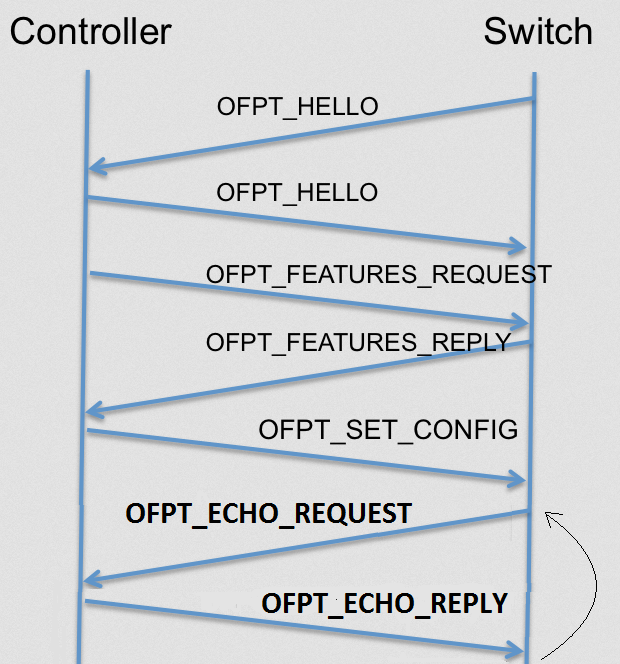
\includegraphics[scale=0.5]{openflow_protocol}
	\centering
	\label{fig:openflow_protocol}
\end{figure}

\begin{figure}[t]
	\caption{Error de comunicación en protocolo de OpenFlow.}
	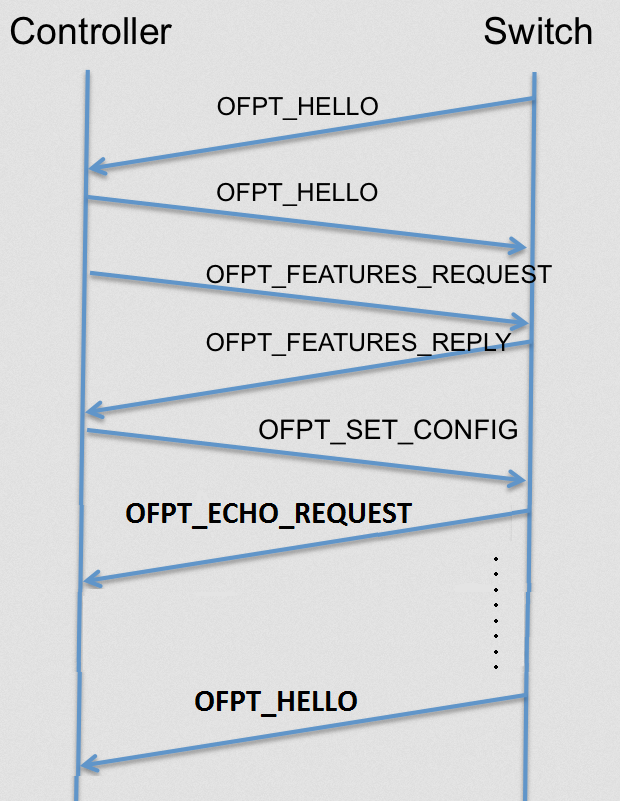
\includegraphics[scale=0.5]{openflow_protocol_error}
	\centering
	\label{fig:openflow_protocol_error}
\end{figure}
De acuerdo al manual de Open vSwitch \cite{ovs-vswitchd-conf}, la variable responsable de este comportamiento es la llamada \textbf{inactivity\_probe}. Se define como el máximo número de mili-segundos que debe esperar el switch antes de enviar un mensaje sonda por inactividad (Echo Request). Si Open vSwitch no se comunica con el controlador por la cantidad especificada de segundos, enviará una sonda, es decir, un mensaje Echo Request. Si la respuesta no es recibida dentro la misma cantidad de mili-segundos adicional, Open vSwitch asume que la conexión se ha finalizado e intenta reconectarse. El valor por defecto para esta variable depende de la implementación, y en el ambiente de trabajo tiene por defecto el número 5000 (5 segundos). Esto quiere decir que si el switch no recibe mensajes del controlador por 10 segundos (5 luego de mandar la sonda) se cerrará la conexión. \\
Lo interesante de esta situación es estudiar por qué el controlador no logra responder a tiempo las sondas de los nodos. Algunas posibles razones son las siguientes:
\begin{itemize}
	\item Congestión en la red de gestión. Es posible que el exceso de nodos genere demasiado tráfico de control, y por ende haya retrasos y/o pérdidas en la red de gestión. Este problema posiblemente estaría presente en un despliegue real de la arquitectura.
	\item Falta de capacidad de cómputo. Dado que este comportamiento se detectó en el entorno virtual y con un número importante de nodos, es posible que el controlador no tenga acceso al poder de cómputo suficiente como para responder a tiempo a todas las sondas. Este sería un problema del entorno virtual, y no sería relevante en una red real.
	\item Incapacidad de Ryu para manejar muchos nodos. En \cite{proyecto-rrap} se menciona que Ryu es un controlador minimalista y académico. Por lo tanto, es posible que no esté diseñado para controlar tantos switches. Si ese fuera el caso, esto sería un obstáculo al desplegar la arquitectura en una red real. 
\end{itemize}
Como solución provisoria, con el propósito de realizar pruebas con las topologias que presentan este problema, se configuró el valor de inactivity\_probe como un número muy alto (45 segundos) de modo de darle al controlador más que suficiente tiempo para responder a las sondas. Sin embargo, esta no es una buena solución ya que en una red real, cuanto más alto esté ese número, más demoraría el controlador en darse cuenta que un switch se desconectó. Se deja para trabajos futuros investigar si esto podría afectar una despliegue real, ya que si lo hace, tendrían que hacerse cambios radicales a la arquitectura.

\subsection{Problema de concurrencia por muchas instancias de OpenVSwitch}
Como se explica en el Proyecto RRAP \cite{proyecto-rrap}, para que las interfaces de red de los nodos funcionen como puertos OpenFlow con dirección IP, no solo se debe crear un puerto en Open vSwitch para cada una, sino que también se debe crear una interfaz virtual con su respectivo puerto. Además, deben crearse flujos para que los paquetes que entran por la interfaz física salgan por su respectiva interfaz virtual, y viceversa.
El siguiente código simplificado muestra como es el proceso de configuración:
\begin{lstlisting}
	ovs-vsctl add-port eth0		#deberia asignar nro de puerto OF 1
	ovs-vsctl add-port eth1		#deberia asignar nro de puerto OF 2
	ovs-vsctl add-port eth2		#deberia asignar nro de puerto OF 3
	ovs-vsctl add-port veth0	#deberia asignar nro de puerto OF 4
	ovs-vsctl add-port veth1	#deberia asignar nro de puerto OF 5
	ovs-vsctl add-port veth2	#deberia asignar nro de puerto OF 6
	
	ovs-ofctl add-flow in_port=1,output:4
	ovs-ofctl add-flow in_port=4,output:1
	ovs-ofctl add-flow in_port=2,output:5
	ovs-ofctl add-flow in_port=5,output:2
	ovs-ofctl add-flow in_port=3,output:6
	ovs-ofctl add-flow in_port=6,output:3
\end{lstlisting}
Cuando se le agrega un puerto, Open vSwitch le asigna automáticamente un número de puerto OpenFlow. La manera en que Open vSwitch hace esa numeración es secuencial, empezando desde 1. Eso quiere decir que, en teoría, si se agregan 3 puertos a Open vSwitch, sus puertos OpenFlow tendrán los números 1, 2 y 3, de acuerdo al orden en que fueron creados. Como se ve en el pseudocódigo, las líneas que agregan los flujos que \enquote{conectan} las interfaces virtuales y físicas asumen que la numeración se hace de esa forma. Está configuración se hace para cada nodo (es decir, para cada instancia de Open vSwitch) y es equivalente a la forma en que se configuran los dispositivos físicos en el prototipo. \\
No se observaron problemas relacionados con esto en topologias chicas de 4 nodos aproximadamente, pero sí en topologias más grandes. Se observó que con más nodos, la numeración de los puertos en Open vSwitch se comportaba de forma impredecible, y no seguía el esquema secuencial que se mencionó anteriormente. Como los flujos que se agregan posteriormente asumen ese determinado orden, eso causa que varias o todas las interfaces del nodo no funcionen. En topologias de entre 10 y 40 nodos ese comportamiento a veces afectaba sólo unos pocos nodos, y en ocasiones no ocurría. Con topologias de 100 nodos aproximadamente, esto ocurría siempre, con más de la mitad de los nodos. Esto llevó a creer que se trataba de un problema de concurrencia por tener muchas instancias de Open vSwitch iniciándose y configurándose al mismo tiempo. \\
Para solucionar este problema se hizo el siguiente cambio:
\begin{lstlisting}
	ovs-vsctl add-port eth0 ofport_request=1
	ovs-vsctl add-port eth1 ofport_request=2
	ovs-vsctl add-port eth2 ofport_request=3
	ovs-vsctl add-port veth0 ofport_request=4
	ovs-vsctl add-port veth1 ofport_request=5
	ovs-vsctl add-port veth2 ofport_request=6
	
	ovs-ofctl add-flow in_port=1,output:4
	ovs-ofctl add-flow in_port=4,output:1
	ovs-ofctl add-flow in_port=2,output:5
	ovs-ofctl add-flow in_port=5,output:2
	ovs-ofctl add-flow in_port=3,output:6
	ovs-ofctl add-flow in_port=6,output:3
\end{lstlisting}
El parámetro opcional \textbf{ofport\_request} permite indicarle a Open vSwitch que número debería asignarle al puerto que se está agregando. Esto soluciona completamente el problema y permite levantar topologias de cualquier tamaño sin problemas. Es importante remarcar que probablemente esto solo afecta al entorno virtual, y no es necesario realizar esta corrección al configurar nodos reales, ya que cada dispositivo ejecuta una única instancia de Open vSwitch y por lo tanto no es probable que se vea este comportamiento. Sin embargo, no se descarta del todo que exista una posibilidad de que esto ocurra, así que se propone el uso de \textbf{ofport\_request} para la configuración de los nodos físicos para eliminar ese riesgo, por más pequeño que sea.

\subsection{Problema de LSDB Sync con muchos nodos}
Como se explicó en el capítulo X, el componente llamado LSDB Sync es el encargado de procesar la información de la base de datos topológica de OSPF y enviarla a las aplicaciones que se ejecutan en el controlador. Este proceso se lleva a cabo en un script escrito en Python, el cual se conecta mediante Telnet con el demonio OSPF, extrae la información topológica y la procesa, y luego la envía al controlador. Se observó que si se está simulando una topología grande (de 100 nodos aproximadamente), la ejecución de este script queda colgada, y no termina. Por lo tanto, la información no se envía nunca al controlador. Para explicar la fuente del problema, es necesario mostrar un pseudocódigo del script:
\begin{lstlisting}
conexion = telnetlib.iniciar_conexion("localhost", PUERTO_OSPFD)
conexion.write(password)
conexion.write("show ip ospf database router")
conexion.write("exit")
info_topologica = conexion.read_all()

procesar_info_topologica
enviar_info_controlador
\end{lstlisting}
La tarea de conectarse con el demonio OSPF mediante Telnet y extraer la información topológica se hace con una librería llamada Telnetlib. La parte que se observó era problemática es la llamada al método \textbf{read\_all()}, usada para leer la información que devuelve el demonio. Al existir muchos nodos, la cantidad de información que deberá devolver el método será extensiva. Se calcula que para topologias de 100 nodos aproximadamente, esa información ronda los 92KB. Aunque no se encontró documentación que lo soporte, el diagnóstico que se hizo es que dicho método no está diseñado para devolver tanta información, y quizás queda colgado por limitaciones de memoria o buffers.

A diferencia de read\_all, que se bloquea hasta terminar de leer, el método \textbf{read\_very\_eager()} lee toda la información que puede pero sin bloquearse \cite{doc-telnetlib}. Con el segundo método, el script no se cuelga, pero sí devuelve información incompleta en ocasiones. Por lo tanto, se adoptó read\_very\_eager como solución al problema, y se agregó una validación al script que compruebe que la información no está incompleta antes de enviarla al controlador.

Se propone un estudio más profundo sobre este tema para trabajos futuros por dos razones. En primer lugar, no se conoce con certeza la razón del comportamiento, y la solución que se adopta lo resuelve pero parcialmente. En segundo lugar, este defecto podría afectar a despliegues reales de la arquitectura RAUFlow.

\subsection{Precaución con MTU}
A diferencia de los problemas mencionados en las secciones anteriores, en esta sección no se discutirá un problema de la arquitectura ni del entorno virtual, sino de una precaución que se debe tener en cuenta a futuro. Como se explica en el capítulo X, las VPN se implementan agregando y quitando etiquetas MPLS a los paquetes que pasan por los switches. Esas etiquetas son de 5 bytes, y dependiendo el camino que debe recorrer, a un paquete se le puede agregar una o dos etiquetas. Es importante tener esto en cuenta ya que impacta en el MTU. Por ejemplo, si se tiene una red Ethernet con un MTU de 1500 bytes, y se envía tráfico TCP sin tener esto en consideración, probablemente se utilice un MSS (Maximum Segment Size) de 1460 bytes, dejando 20 bytes para el cabezal IP y 20 más para el TCP. En ese caso, el tráfico no pasa por la red, ya que cuando el switch de borde recibe los paquetes y les asigna las etiquetas MPLS que corresponden, los mismos pasan a tener más de 1500 bytes, y por lo tanto no se envían. Para solucionarlo, se debe reducir el MSS a 1455 en caso de que el camino sea de un salto (se le asigna una etiqueta), y a 1450 en caso contrario (se asignan dos etiquetas).

\chapter{Pruebas de escala}

% **************************** Define Graphics Path **************************
\graphicspath{{Chapter4/Figs/}}

Con el entorno de simulación construido, el siguiente objetivo es realizar pruebas de escala sobre la arquitectura. Se realizan dos tipos de pruebas de escala: (a) verificar cómo funciona la arquitectura para topologias de escala, (b) realizar estudios de escala sobre la cantidad de servicios que soporta. En este capítulo se explicará el propósito de cada prueba, las condiciones bajo las cuales se ejecuta cada una de ellas (topologias, tipos de tráfico, etc) y por último, los resultados que arrojan. Las pruebas fueron realizadas en el servidor del Instituto de Computación, con una máquina virtual Lubuntu 14.04 sobre KVM, con 32GB de RAM y un procesador AMD Opteron 23xx.

\section{Topologias de escala}
El objetivo de estas pruebas es aplicar topologias de diferentes tamaños y características a la arquitectura y estudiar el proceso de creación de las redes privadas virtuales en cada realidad.

Las topologias utilizadas se listan a continuación:
\begin{itemize}
	\item \textbf{Básica}: 4 nodos en topología de full mesh. Es la utilizada en el prototipo físico. Figura \ref{fig:basic_topology}.
	\item \textbf{Chica}: topología arbitraria de 11 nodos (fuente: Topology Zoo). Figura \ref{fig:small_topology}.
	\item \textbf{Mediana}: topología arbitraria de 45 nodos (fuente: Topology Zoo). Figura \ref{fig:medium_topology}.
	\item \textbf{Grande}: topología de tipo arborescente compuesta por 105 nodos. Figura \ref{fig:large_topology}
\end{itemize}

Todas las topologias tienen las siguientes características:
\begin{itemize}
	\item Tienen un conjunto de RAUSwitch, conectados de acuerdo a lo que dicte la topología.
	\item Existen dos subredes cliente, implementadas por un QuaggaRouter y un RAUHost cada una (recordar las clases del entorno virtual). El RAUHost representa la computadora que utiliza el usuario final para conectarse a la red, y QuaggaRouter representa el router legacy que conecta la subred del usuario a la red SDN. Los RAUHost serán los remitentes y destinatarios del tráfico que pasará por la red. Esos datos se generarán con el comando \textit{ping} y la herramienta \textit{iperf}. Estas dos subredes tendrán una ubicación variable en cada topología, ya que se probará con distintos caminos entre ellas. Por esta razón, se omiten en las imágenes de las topologias.
	\item El controlador se conecta con un switch virtual genérico (implementado por la clase Switch de Mininet, en el modo \textit{standalone}), el cual se conecta con los RAUSwitch. Esta será la red de gestión. Por simplicidad, dicha red se omite en las imágenes.
\end{itemize}

\begin{figure}[H]
	\caption{Topología de prueba básica}
	\includegraphics[scale=0.6]{basic_topology}
	\centering
	\label{fig:basic_topology}
\end{figure}

\begin{figure}[H]
	\caption{Topología de prueba chica}
	\includegraphics[scale=0.4]{small_topology}
	\centering
	\label{fig:small_topology}
\end{figure}

\begin{figure}[H]
	\caption{Topología de prueba grande}
	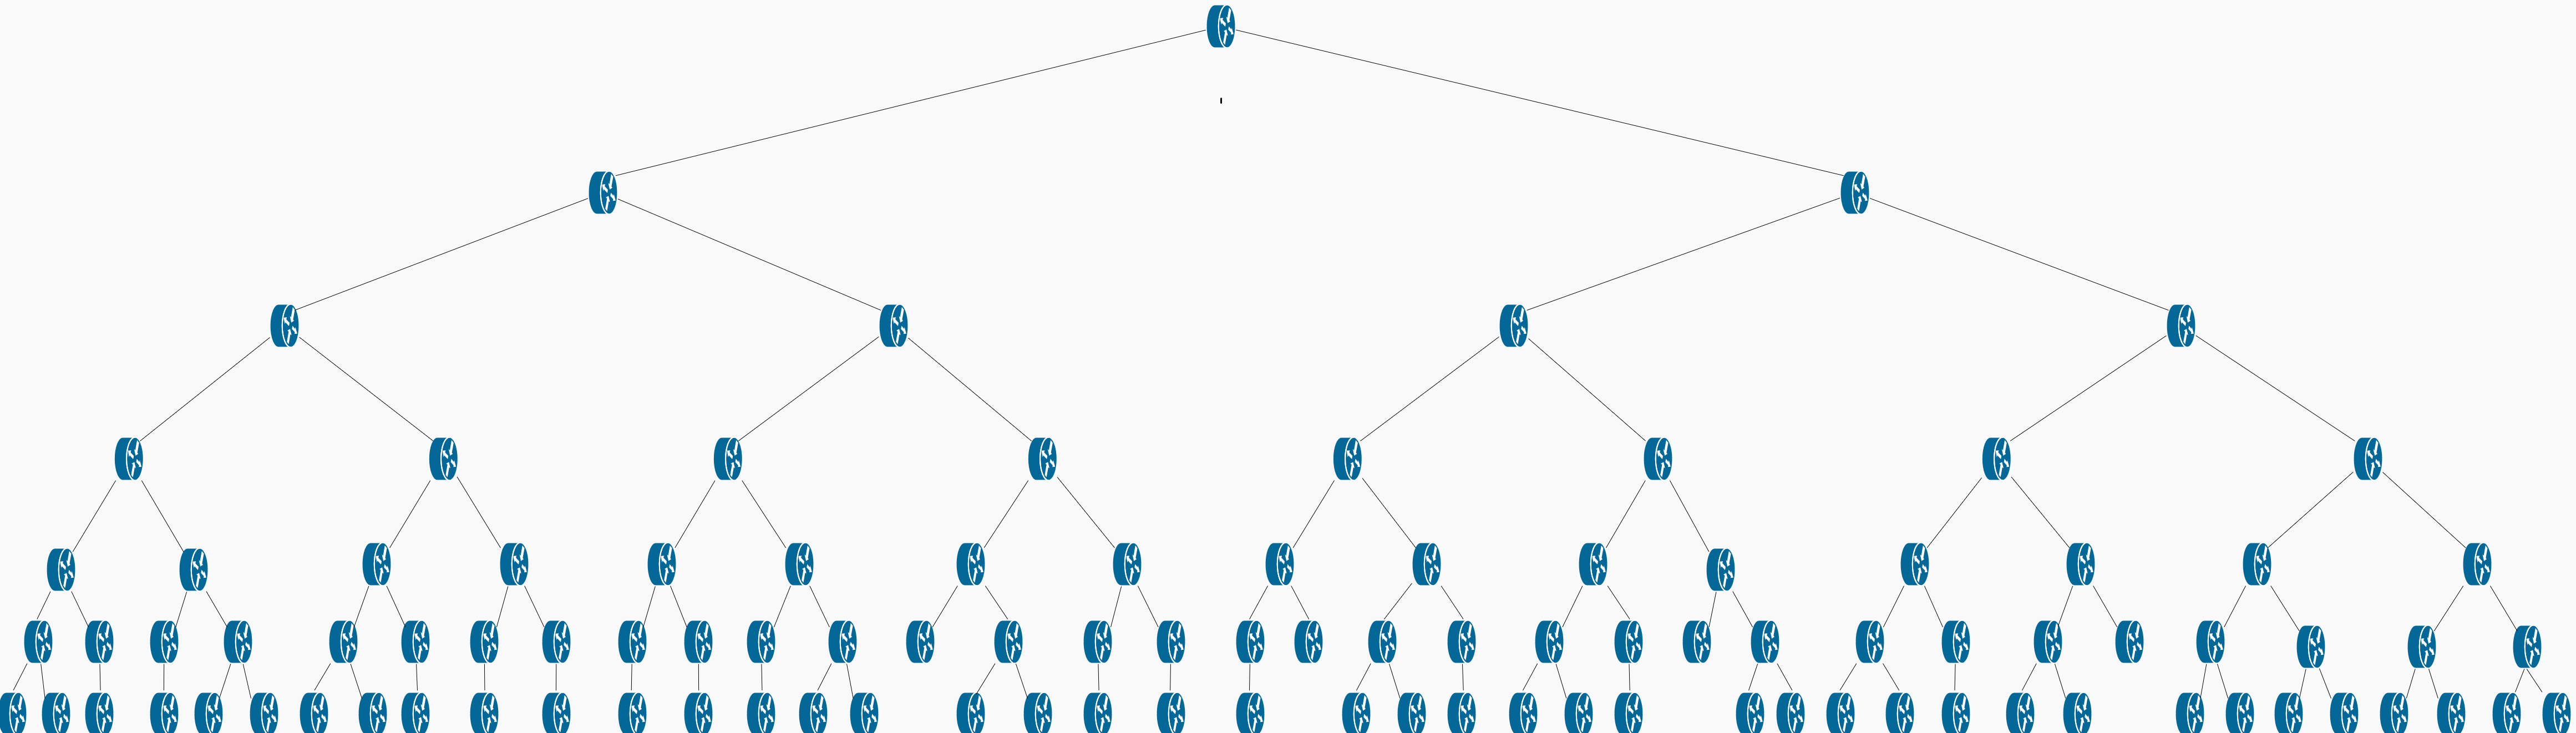
\includegraphics[width=\textwidth,height=\textheight,keepaspectratio]{large_topology}
	\centering
	\label{fig:large_topology}
\end{figure}

\begin{figure}[H]
	\caption{Topología de prueba mediana}
	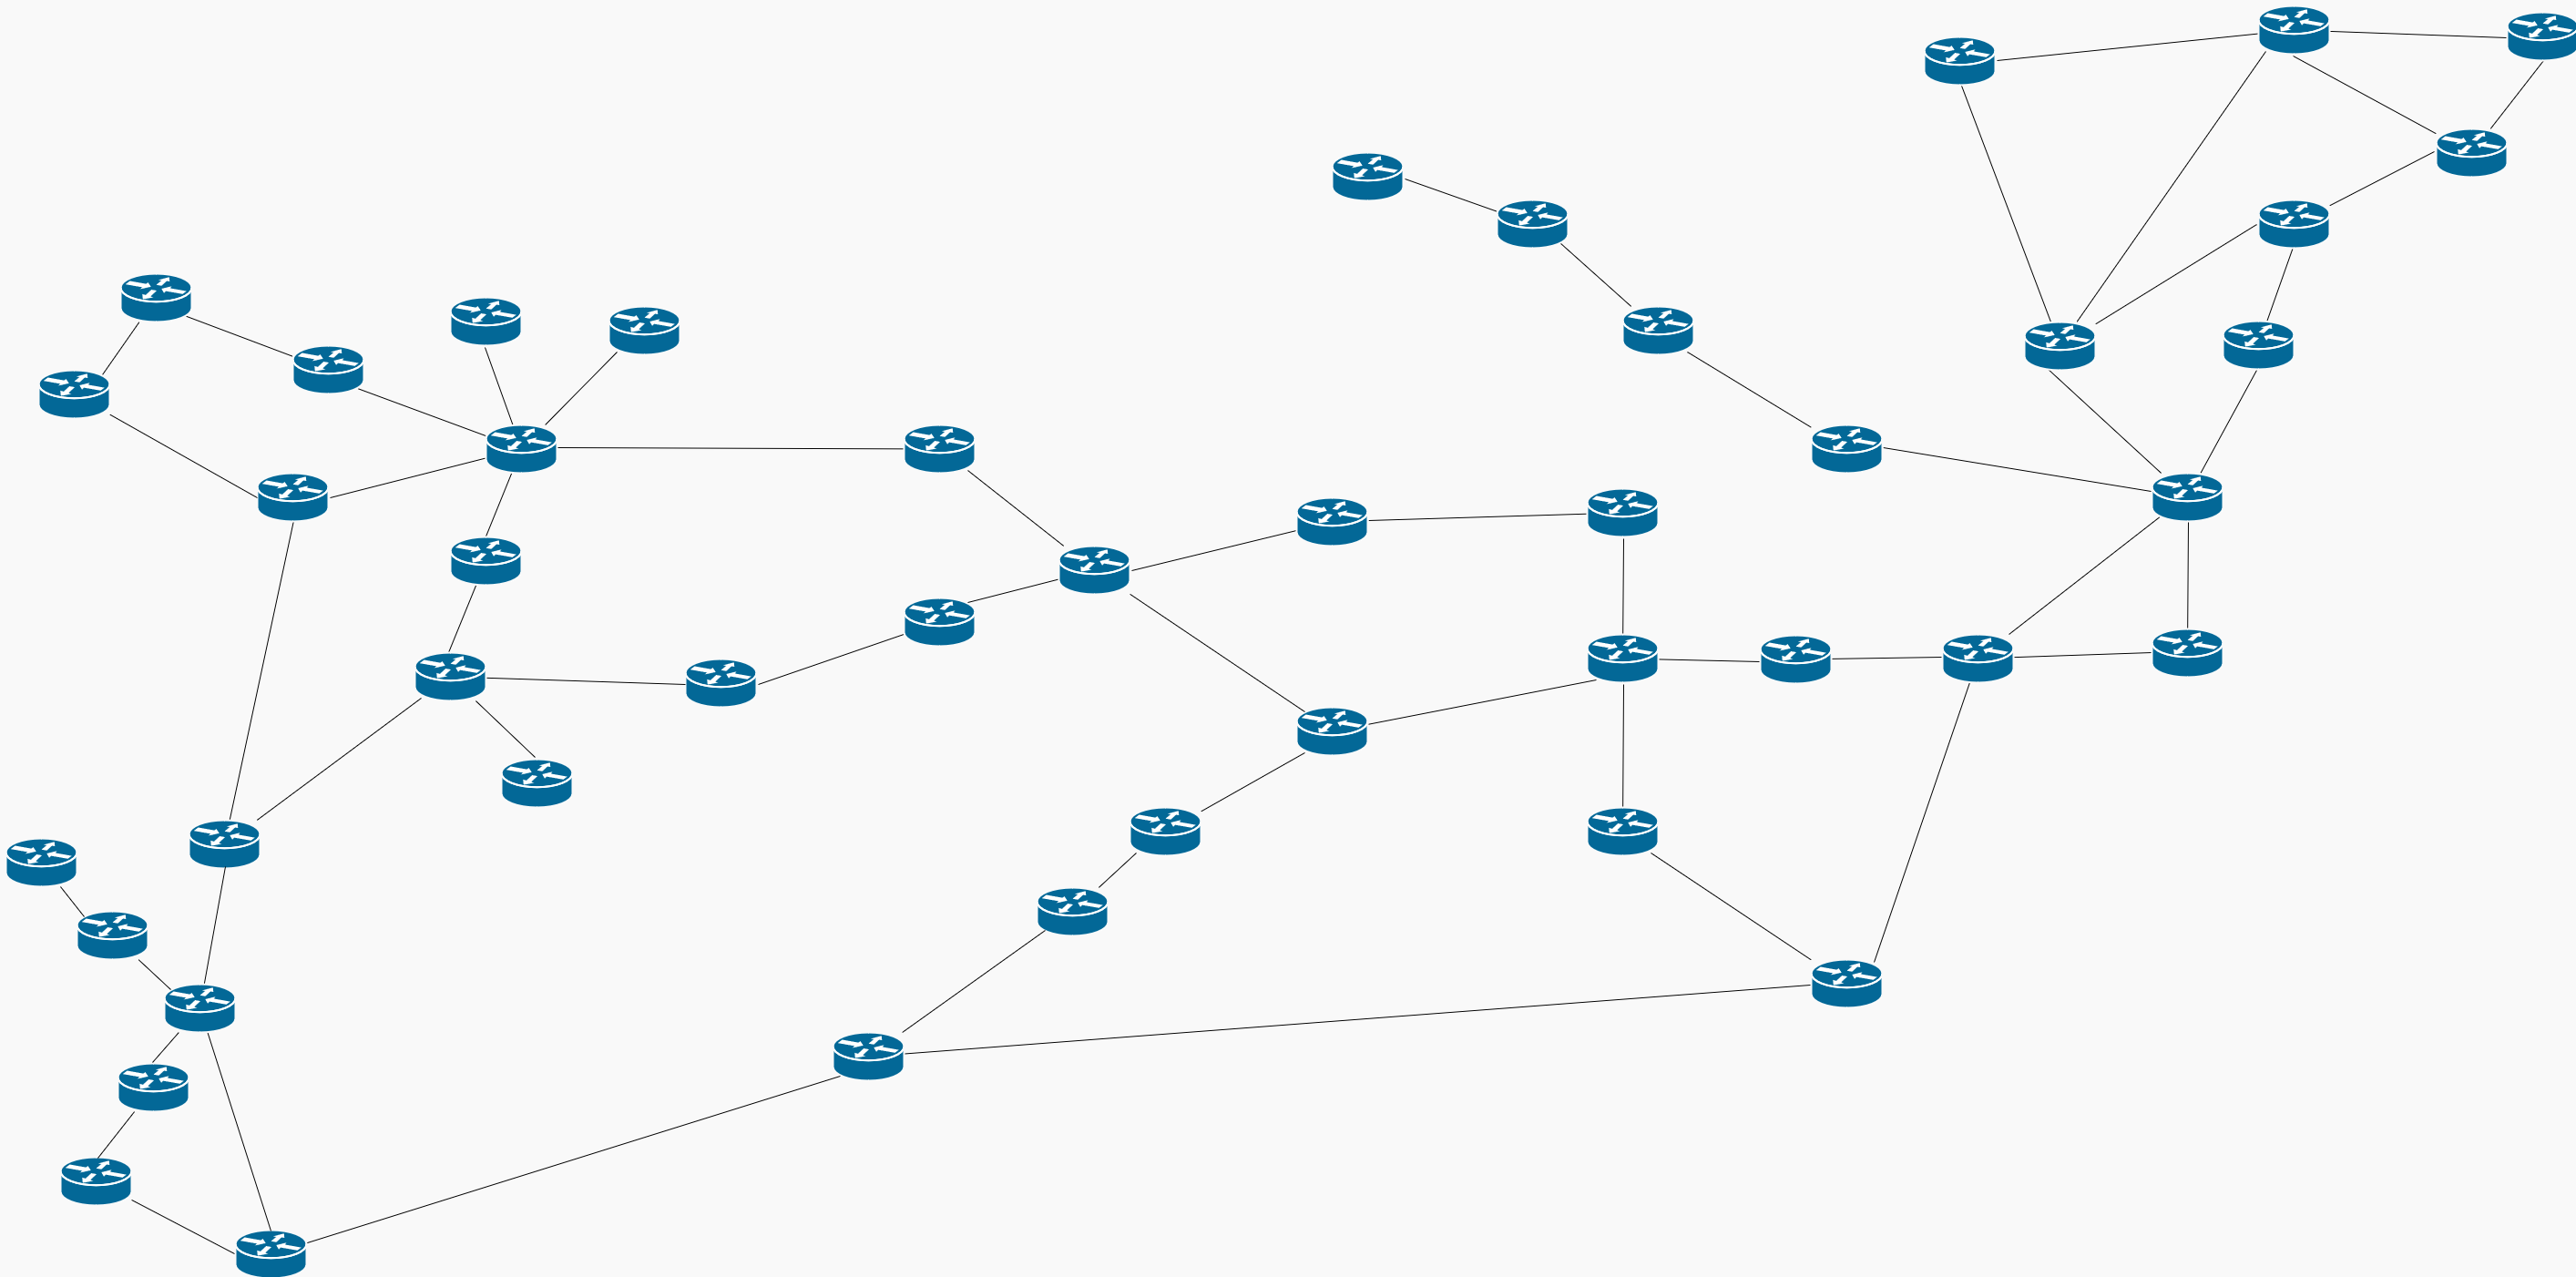
\includegraphics[width=\textwidth,height=\textheight,keepaspectratio]{medium_topology}
	\centering
	\label{fig:medium_topology}
\end{figure}

Es importante tener en cuenta que realizar esta serie de pruebas es posible gracias al proceso de verificación funcional explicado en la sección 3.5. En ella se explica la detección y corrección de algunos problemas de escalabilidad tanto del entorno virtual como de la arquitectura RAUFlow misma. Por lo tanto, estas pruebas se pueden considerar como una continuación del estudio de escalabilidad presentado en dicha sección.

\subsection{Escenario}
El objetivo es estudiar como impacta el tamaño de la topología y el largo del camino en el tiempo que demora la arquitectura en establecer una VPN entre dos subredes cliente. Se espera que ese tiempo sea influenciado en gran medida por dos factores: el tiempo que demora el controlador en calcular el camino óptimo y el tiempo que demora en configurar los flujos en cada nodo del camino. Dado que los servicios se crean enviando pedidos HTTP POST al controlador (y se deben enviar dos por cada VPN, uno de ida y uno de vuelta), el tiempo de creación de los mismos se medirá como el tiempo que demore el controlador en devolver las respuestas HTTP indicando que fueron creados con éxito (esta información está disponible en los logs). Para lograr resultados representativos y reducir el margen de error, en lugar de crear una VPN y medir su tiempo solamente, se realizan cuatro ejecuciones y se calculan las métricas estadísticas relevantes. Para agilizar la ejecución de esta prueba se utiliza un script en Python que manda los pedidos HTTP POST al controlador para crear las VPN, y de este modo no hay necesidad de hacerlo manualmente a través de la interfaz web.

\newcolumntype{?}{!{\vrule width 3pt}}
\newcolumntype{M}[1]{>{\centering\arraybackslash}m{#1}}
\begin{table}
	\caption{Tiempo que demora el controlador en dar de alta VPNs. El tiempo se mide en ms. Los valores de color marrón  corresponden a la VPN de capa 2, y los azules a la de capa 3.}
	\centering
	\scriptsize
	\bgroup
	\setlength{\tabcolsep}{.17em}
	\begin{tabular}{M{1.1cm}? M{0.8cm} | M{1.7cm} | M{1.7cm} | M{1.7cm} | M{1.7cm} | M{1.5cm} | M{1.4cm} | M{1.3cm} | M{1.3cm} |@{}m{0pt}@{}}
		\Xhline{5\arrayrulewidth}
		Topología & Largo del camino & Ejecución 1 (ms) & Ejecución 2 (ms) & Ejecución 3 (ms) & Ejecución 4 (ms) & Media (ms) & Mediana (ms) & Desv. Estándar (ms) & CV & \\
		\hline
		Básica & 1 & \textcolor{brown}{188} / \textcolor{blue}{14} & \textcolor{brown}{188} / \textcolor{blue}{23} & \textcolor{brown}{199} / \textcolor{blue}{15} & \textcolor{brown}{188} / \textcolor{blue}{15} & \textcolor{brown}{191} / \textcolor{blue}{17} & \textcolor{brown}{188} / \textcolor{blue}{15} & \textcolor{brown}{6} / \textcolor{blue}{4} & \textcolor{brown}{0.03} / \textcolor{blue}{0.24} & \\[3ex]
		\Xhline{5\arrayrulewidth}
		& 1 & \textcolor{brown}{155} / \textcolor{blue}{29} & \textcolor{brown}{208} / \textcolor{blue}{22} & \textcolor{brown}{351} / \textcolor{blue}{19} & \textcolor{brown}{220} / \textcolor{blue}{18} & \textcolor{brown}{234} / \textcolor{blue}{22} & \textcolor{brown}{214} / \textcolor{blue}{21} & \textcolor{brown}{83} / \textcolor{blue}{5} & \textcolor{brown}{0.35} / \textcolor{blue}{0.23} & \\[3ex] \cline{2-10}
		& 2 & \textcolor{brown}{241} / \textcolor{blue}{25} & \textcolor{brown}{309} / \textcolor{blue}{27} & \textcolor{brown}{317} / \textcolor{blue}{31} & \textcolor{brown}{317} / \textcolor{blue}{29} & \textcolor{brown}{296} / \textcolor{blue}{28} & \textcolor{brown}{313} / \textcolor{blue}{28} & \textcolor{brown}{37} / \textcolor{blue}{3} & \textcolor{brown}{0.13} / \textcolor{blue}{0.11} & \\[3ex] \cline{2-10}
		Chica & 4 & \textcolor{brown}{269} / \textcolor{blue}{52} & \textcolor{brown}{298} / \textcolor{blue}{42} & \textcolor{brown}{327} / \textcolor{blue}{43} & \textcolor{brown}{301} / \textcolor{blue}{39} & \textcolor{brown}{299} / \textcolor{blue}{44} & \textcolor{brown}{300} / \textcolor{blue}{43} & \textcolor{brown}{24} / \textcolor{blue}{6} & \textcolor{brown}{0.08} / \textcolor{blue}{0.14} & \\[3ex] \cline{2-10}
		& 6 & \textcolor{brown}{257} / \textcolor{blue}{42} & \textcolor{brown}{320} / \textcolor{blue}{55} & \textcolor{brown}{348} / \textcolor{blue}{56} & \textcolor{brown}{326} / \textcolor{blue}{57} & \textcolor{brown}{313} / \textcolor{blue}{53} & \textcolor{brown}{323} / \textcolor{blue}{56} & \textcolor{brown}{39} / \textcolor{blue}{7} & \textcolor{brown}{0.12} / \textcolor{blue}{0.13} & \\[3ex] \cline{2-10}
		& 8 & \textcolor{brown}{285} / \textcolor{blue}{51} & \textcolor{brown}{333} / \textcolor{blue}{64} & \textcolor{brown}{337} / \textcolor{blue}{64} & \textcolor{brown}{342} / \textcolor{blue}{60} & \textcolor{brown}{324} / \textcolor{blue}{60} & \textcolor{brown}{335} / \textcolor{blue}{62} & \textcolor{brown}{26} / \textcolor{blue}{6} & \textcolor{brown}{0.08} / \textcolor{blue}{0.10} & \\[3ex] \cline{2-10}
		\Xhline{5\arrayrulewidth}
		& 1 & \textcolor{brown}{254} / \textcolor{blue}{101} & \textcolor{brown}{318} / \textcolor{blue}{92} & \textcolor{brown}{355} / \textcolor{blue}{110} & \textcolor{brown}{318} / \textcolor{blue}{110} & \textcolor{brown}{311} / \textcolor{blue}{103} & \textcolor{brown}{318} / \textcolor{blue}{106} & \textcolor{brown}{42} / \textcolor{blue}{9} & \textcolor{brown}{0.14} / \textcolor{blue}{0.09} & \\[3ex] \cline{2-10}
		& 2 & \textcolor{brown}{567} / \textcolor{blue}{104} & \textcolor{brown}{746} / \textcolor{blue}{134} & \textcolor{brown}{520} / \textcolor{blue}{112} & \textcolor{brown}{611} / \textcolor{blue}{127} & \textcolor{brown}{611} / \textcolor{blue}{119} & \textcolor{brown}{589} / \textcolor{blue}{120} & \textcolor{brown}{97} / \textcolor{blue}{14} & \textcolor{brown}{0.16} / \textcolor{blue}{0.12} & \\[3ex] \cline{2-10}
		& 4 & \textcolor{brown}{372} / \textcolor{blue}{129} & \textcolor{brown}{504} / \textcolor{blue}{105} & \textcolor{brown}{498} / \textcolor{blue}{135} & \textcolor{brown}{438} / \textcolor{blue}{145} & \textcolor{brown}{453} / \textcolor{blue}{129} & \textcolor{brown}{468} / \textcolor{blue}{132} & \textcolor{brown}{62} / \textcolor{blue}{17} & \textcolor{brown}{0.14} / \textcolor{blue}{0.13} & \\[3ex] \cline{2-10}
		Mediana & 6 & \textcolor{brown}{364} / \textcolor{blue}{126} & \textcolor{brown}{397} / \textcolor{blue}{187} & \textcolor{brown}{675} / \textcolor{blue}{164} & \textcolor{brown}{529} / \textcolor{blue}{153} & \textcolor{brown}{491} / \textcolor{blue}{158} & \textcolor{brown}{463} / \textcolor{blue}{159} & \textcolor{brown}{142} / \textcolor{blue}{25} & \textcolor{brown}{0.29} / \textcolor{blue}{0.16} & \\[3ex] \cline{2-10}
		& 8 & \textcolor{brown}{436} / \textcolor{blue}{130} & \textcolor{brown}{515} / \textcolor{blue}{271} & \textcolor{brown}{529} / \textcolor{blue}{202} & \textcolor{brown}{787} / \textcolor{blue}{179} & \textcolor{brown}{567} / \textcolor{blue}{196} & \textcolor{brown}{522} / \textcolor{blue}{191} & \textcolor{brown}{152} / \textcolor{blue}{59} & \textcolor{brown}{0.27} / \textcolor{blue}{0.30} & \\[3ex] \cline{2-10}
		& 10 & \textcolor{brown}{414} / \textcolor{blue}{181} & \textcolor{brown}{548} / \textcolor{blue}{197} & \textcolor{brown}{485} / \textcolor{blue}{214} & \textcolor{brown}{477} / \textcolor{blue}{191} & \textcolor{brown}{481} / \textcolor{blue}{196} & \textcolor{brown}{481} / \textcolor{blue}{194} & \textcolor{brown}{55} / \textcolor{blue}{14} & \textcolor{brown}{0.11} / \textcolor{blue}{0.07} & \\[3ex] \cline{2-10}
		& 12 & \textcolor{brown}{441} / \textcolor{blue}{289} & \textcolor{brown}{519} / \textcolor{blue}{152} & \textcolor{brown}{613} / \textcolor{blue}{154} & \textcolor{brown}{571} / \textcolor{blue}{178} & \textcolor{brown}{536} / \textcolor{blue}{193} & \textcolor{brown}{545} / \textcolor{blue}{166} & \textcolor{brown}{74} / \textcolor{blue}{65} & \textcolor{brown}{0.14} / \textcolor{blue}{0.34} & \\[3ex] \cline{2-10}
		\Xhline{5\arrayrulewidth}
		& 1 & \textcolor{brown}{425} / \textcolor{blue}{483} & \textcolor{brown}{940} / \textcolor{blue}{325} & \textcolor{brown}{573} / \textcolor{blue}{581} & \textcolor{brown}{428} / \textcolor{blue}{282} & \textcolor{brown}{592} / \textcolor{blue}{418} & \textcolor{brown}{501} / \textcolor{blue}{404} & \textcolor{brown}{242} / \textcolor{blue}{139} & \textcolor{brown}{0.41} / \textcolor{blue}{0.33} & \\[3ex] \cline{2-10}
		& 2 & \textcolor{brown}{642} / \textcolor{blue}{810} & \textcolor{brown}{457} / \textcolor{blue}{223} & \textcolor{brown}{1044} / \textcolor{blue}{319} & \textcolor{brown}{2671} / \textcolor{blue}{1346} & \textcolor{brown}{1204} / \textcolor{blue}{675} & \textcolor{brown}{843} / \textcolor{blue}{565} & \textcolor{brown}{1009} / \textcolor{blue}{516} & \textcolor{brown}{0.99} / \textcolor{blue}{0.76} & \\[3ex] \cline{2-10}
		& 4 & \textcolor{brown}{1692} / \textcolor{blue}{1000} & \textcolor{brown}{2457} / \textcolor{blue}{2209} & \textcolor{brown}{1543} / \textcolor{blue}{1070} & \textcolor{brown}{1613} / \textcolor{blue}{668} & \textcolor{brown}{1826} / \textcolor{blue}{1237} & \textcolor{brown}{1653} / \textcolor{blue}{1035} & \textcolor{brown}{425} / \textcolor{blue}{672} & \textcolor{brown}{0.23} / \textcolor{blue}{0.54} & \\[3ex] \cline{2-10}
		Grande & 6 & \textcolor{brown}{1669} / \textcolor{blue}{722} & \textcolor{brown}{1254} / \textcolor{blue}{1016} & \textcolor{brown}{1048} / \textcolor{blue}{476} & \textcolor{brown}{2678} / \textcolor{blue}{569} & \textcolor{brown}{1662} / \textcolor{blue}{696} & \textcolor{brown}{1462} / \textcolor{blue}{646} & \textcolor{brown}{725} / \textcolor{blue}{236} & \textcolor{brown}{0.44} / \textcolor{blue}{0.34} & \\[3ex] \cline{2-10}
		& 8 & \textcolor{brown}{1516} / \textcolor{blue}{2182} & \textcolor{brown}{2273} / \textcolor{blue}{608} & \textcolor{brown}{3482} / \textcolor{blue}{856} & \textcolor{brown}{3496} / \textcolor{blue}{748} & \textcolor{brown}{2692} / \textcolor{blue}{1099} & \textcolor{brown}{2878} / \textcolor{blue}{802} & \textcolor{brown}{972} / \textcolor{blue}{729} & \textcolor{brown}{0.36} / \textcolor{blue}{0.66} & \\[3ex] \cline{2-10}
		& 10 & \textcolor{brown}{493} / \textcolor{blue}{449} & \textcolor{brown}{775} / \textcolor{blue}{638} & \textcolor{brown}{784} / \textcolor{blue}{563} & \textcolor{brown}{966} / \textcolor{blue}{570} & \textcolor{brown}{755} / \textcolor{blue}{555} & \textcolor{brown}{780} / \textcolor{blue}{567} & \textcolor{brown}{195} / \textcolor{blue}{78} & \textcolor{brown}{0.26} / \textcolor{blue}{0.14} & \\[3ex] \cline{2-10}
		& 12 & \textcolor{brown}{1843} / \textcolor{blue}{594} & \textcolor{brown}{3438} / \textcolor{blue}{1422} & \textcolor{brown}{1791} / \textcolor{blue}{1018} & \textcolor{brown}{2848} / \textcolor{blue}{849} & \textcolor{brown}{2480} / \textcolor{blue}{971} & \textcolor{brown}{2346} / \textcolor{blue}{934} & \textcolor{brown}{803} / \textcolor{blue}{348} & \textcolor{brown}{0.32} / \textcolor{blue}{0.36} & \\[3ex] \cline{2-10}
		\Xhline{5\arrayrulewidth}
	\end{tabular}
	\egroup
	\label{table:tiempos_por_topologia}
\end{table}

La tabla \ref{table:tiempos_por_topologia} muestra los resultados obtenidos en el escenario. En ella se muestran los tiempos obtenidos para cada topología y largo de camino. Cada caso fue ejecutado cuatro veces, y para cada conjunto de ejecuciones se calcula la media, mediana, desviación estándar y coeficiente de variación (CV).

El primer dato que se puede extraer de los resultados obtenidos es que hay una diferencia de tiempo significativa entre una VPN de capa 2 y una de capa 3. La explicación de este comportamiento se encuentra en el algoritmo de distribución de etiquetas MPLS, explicado en la sección 5.5.4 de \cite{proyecto-rrap}. En ella se explica el problema de que, cuando un paquete entra a la red, su ethertype es sustituido por el ethertype correspondiente al protocolo MPLS. Esto implica que cuando el paquete sale de la red, es necesario de alguna forma obtener el ethertype original del mismo. Como explica la documentación de RRAP, en la VPN de capa 3 esto se resuelve haciendo que el usuario indique el ethertype del servicio cuando lo crea. Por otro lado, dado que el tráfico de una VPN de capa 2 puede ser de cualquier ethertype, la solución adoptada es, por cada servicio de capa 2, instalar 42 flujos, uno por cada ethertype posible. De esta forma, cuando el paquete sale de la red, se le asigna el ethertype que corresponda al flujo que utilizó. Desde el punto de vista del tiempo, es esperable que crear una VPN de capa 2 requiera más tiempo que una de capa 3, ya que debe instalar muchos más flujos en los nodos de su camino.

También se puede observar que los tiempos tienden a incrementarse a medida que el camino por el que pasa la VPN es mayor. Esto se debe principalmente a que mientras más nodos haya en el camino, más flujos deben instalarse. Se observa una diferencia de tiempo más acentuada entre el camino de largo 1 y el de 2. Esto se debe a que cuando la VPN pasa por un camino de largo uno el controlador debe configurar sólo un nivel de etiquetas MPLS, mientras que si el camino es de largo mayor, corresponden dos niveles de etiquetas. Esto requiere más tiempo de computo, e instalar al menos un flujo adicional.

Si se comparan los resultados entre cada topología, también hay observaciones importantes. En primer lugar, se puede ver que para caminos de igual largo, si la topología es más grande entonces se necesita más tiempo para crear la VPN. Ese comportamiento se explica con los siguientes puntos:
\begin{itemize}
	\item Si la topología tiene más nodos, entonces el algoritmo Dijkstra que calcula el camino óptimo va a demorar más tiempo en converger.
	\item A medida que hay más RAUSwitch en la topología, la red de gestión tiene más tráfico por la mensajería generada por OpenFlow. Esto puede llevar a congestión en dicha red. Los flujos correspondientes a cada nodo son instalados mediante mensajes OpenFlow que envía el controlador a través de la red de gestión, y si esos mensajes experimentan retrasos o pérdidas, entonces eso significa un retraso en la creación de la VPN. Este fenómeno también se explora en la sección 3.5.2.
	\item Como se está usando un emulador, tener más nodos implica que el procesador anfitrión debe repartir el tiempo de cómputo entre más procesos. Naturalmente, esto resulta en una lentitud generalizada que afecta a toda la red virtual. A diferencia de los puntos anteriores, este fenómeno no se observaría en un despliegue real de la red, así que es relevante solo en este ambiente de pruebas.
\end{itemize}
Los dos últimos puntos también ayudan a explicar otro detalle importante que muestran las tablas: el coeficiente de variación (CV). Se puede observar que este valor es mayor a medida que crece la topología, y que incluso llega a 0.99 (o 99\%) cuando se realizaron las ejecuciones en la topología grande. Esto implica que a medida que la topología crece, la variabilidad de los tiempos que se miden es mayor, y por lo tanto son menos confiables.
El segundo punto puede explicar esto porque si hay congestión en la red, entonces la variabilidad del RTT (round-trip time) puede ser mayor. El tercer punto también puede influir en un CV más alto, ya que es posible que una sobrecarga en la CPU introduzca variabilidad al tiempo de CPU que recibe cada proceso, o quizás también una variabilidad en las tareas que puede desempeñar un proceso dado un determinado tiempo de CPU. \\

Con el objetivo de hacer un análisis más fino sobre el tiempo de creación de las VPNs, se repitieron las pruebas pero agregando modificaciones al código del controlador que permitan analizar cuánto tiempo dedica a cada parte del proceso. Se identificaron tres partes fundamentales: el cálculo del camino óptimo, todo lo relacionado al cálculo y manejo de las etiquetas MPLS, y la instalación de los flujos OpenFlow. La ejecución de esas tres tareas abarca la mayoría (más del 90\%) del tiempo de creación de una VPN. Las modificaciones en el código consistieron de agregar \textit{timestamps}\footnote{Marca temporal que indica la hora en la que se lleva a cabo un evento.} en las partes claves del código. Luego, analizando el log del controlador se hace la resta de los diferentes timestamps para determinar cuánto tiempo se tomó para cada tarea. Es importante tener en cuenta que este método tiene un margen de error no despreciable, ya que está a la merced del tiempo de CPU que se le asigna al controlador. De hecho, algunas ejecuciones fueron descartadas de los resultados ya que se alejan demasiado del resto, probablemente porque la CPU fue asignada durante la creación de una VPN a otros procesos por demasiado tiempo.

Las gráficas en las figuras \ref{fig:gráfica_tiempo_chica}, \ref{fig:gráfica_tiempo_mediana} y \ref{fig:gráfica_tiempo_grande} a continuación muestran, para cada topología, cómo se descompone el tiempo de ejecución para cada largo de camino. Se omite la de la topología básica ya que sólo permite crear VPNs de largo 1. Cada punto en la gráfica indica el porcentaje del tiempo total que se necesitó para llevar a cabo una de las tres tareas ya mencionadas (cálculo del camino, manejo de etiquetas, instalación de flujos OpenFlow). Cada porcentaje se mide en base al promedio de 8 ejecuciones (descartando las ejecuciones que arrojan valores muy alejados del resto).

\begin{figure}[H]
	\caption{Distribución del tiempo de creación de VPNs en la topología chica}
	\centering
	\label{fig:gráfica_tiempo_chica}
	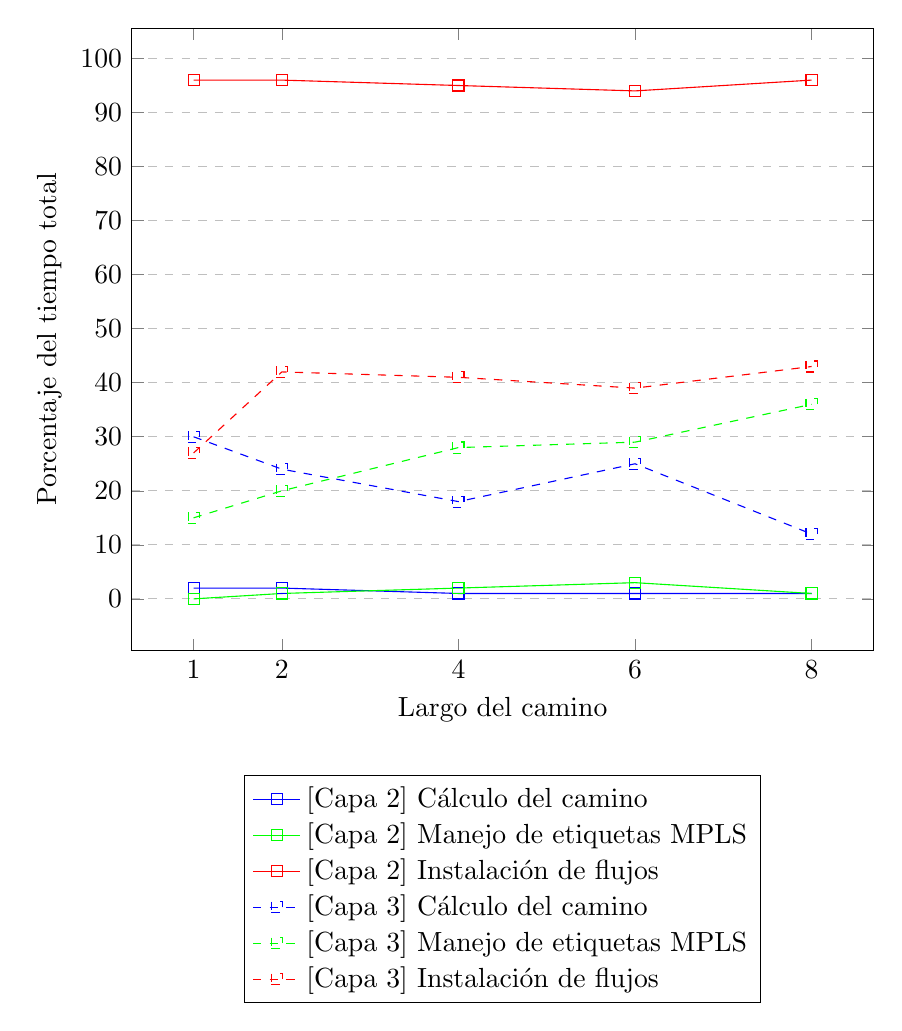
\begin{tikzpicture}
	\begin{axis}[
	xlabel={Largo del camino},
	ylabel={Porcentaje del tiempo total},
	xtick={0,1,2,4,6,8,10,12},
	ytick={0,10,20,30,40,50,60,70,80,90,100},
	scaled x ticks = false,
	x tick label style={/pgf/number format/fixed},
	legend style={at={(0.5,-0.2)},anchor=north},
	ymajorgrids=true,
	grid style=dashed,
	width=11cm,
	legend cell align=left,
	]
	\addplot[
	color=blue,
	mark=square,
	]
	coordinates {
		(1,2)(2,2)(4,1)(6,1)(8,1)
	};
	\addlegendentry{[Capa 2] Cálculo del camino}
	\addplot[
	color=green,
	mark=square,
	]
	coordinates {
		(1,0)(2,1)(4,2)(6,3)(8,1)
	};
	\addlegendentry{[Capa 2] Manejo de etiquetas MPLS}
	\addplot[
	color=red,
	mark=square,
	]
	coordinates {
		(1,96)(2,96)(4,95)(6,94)(8,96)
	};
	\addlegendentry{[Capa 2] Instalación de flujos}
	\addplot[
	color=blue,
	mark=square,
	dashed,
	]
	coordinates {
		(1,30)(2,24)(4,18)(6,25)(8,12)
	};
	\addlegendentry{[Capa 3] Cálculo del camino}
	\addplot[
	color=green,
	mark=square,
	dashed,
	]
	coordinates {
		(1,15)(2,20)(4,28)(6,29)(8,36)
	};
	\addlegendentry{[Capa 3] Manejo de etiquetas MPLS}
	\addplot[
	color=red,
	mark=square,
	dashed,
	]
	coordinates {
		(1,27)(2,42)(4,41)(6,39)(8,43)
	};
	\addlegendentry{[Capa 3] Instalación de flujos}
	\end{axis}
	\end{tikzpicture}
\end{figure}

\begin{figure}[H]
	\caption{Distribución del tiempo de creación de VPNs en la topología mediana}
	\centering
	\label{fig:gráfica_tiempo_mediana}
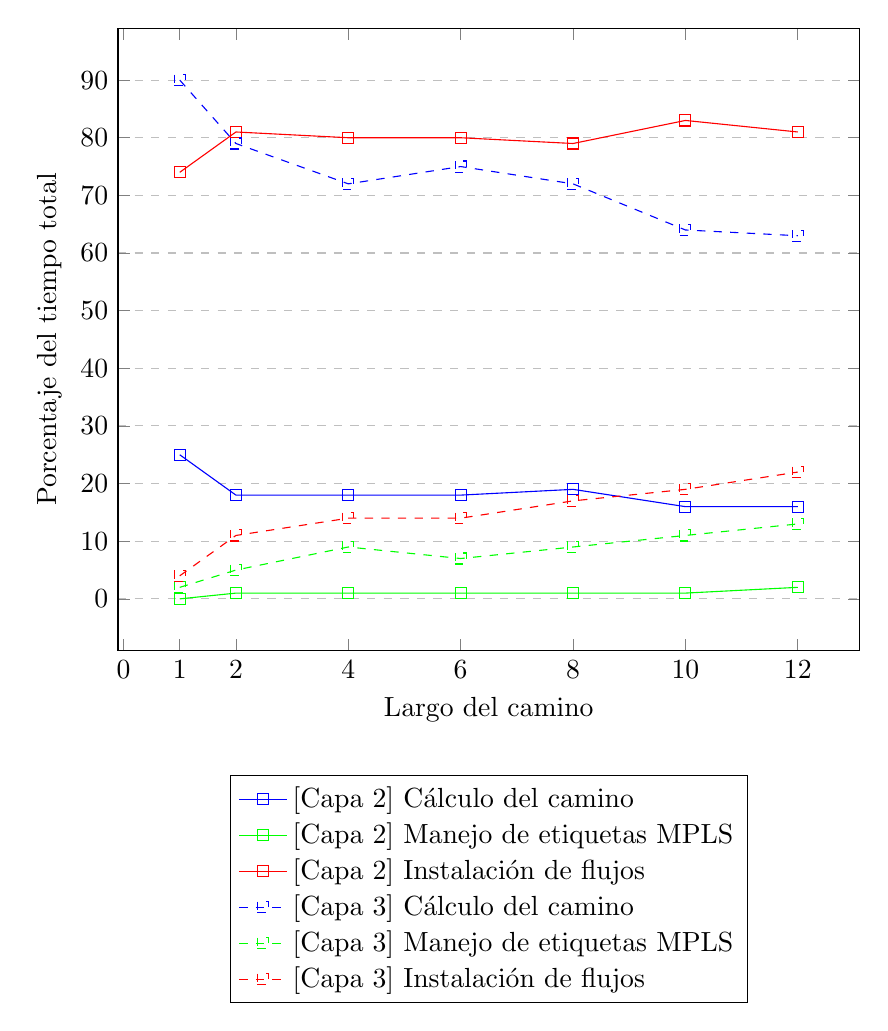
\begin{tikzpicture}
\begin{axis}[
xlabel={Largo del camino},
ylabel={Porcentaje del tiempo total},
xtick={0,1,2,4,6,8,10,12},
ytick={0,10,20,30,40,50,60,70,80,90,100},
scaled x ticks = false,
x tick label style={/pgf/number format/fixed},
legend style={at={(0.5,-0.2)},anchor=north},
ymajorgrids=true,
grid style=dashed,
width=11cm,
legend cell align=left,
]
\addplot[
color=blue,
mark=square,
]
coordinates {
	(1,25)(2,18)(4,18)(6,18)(8,19)(10,16)(12,16)
};
\addlegendentry{[Capa 2] Cálculo del camino}
\addplot[
color=green,
mark=square,
]
coordinates {
	(1,0)(2,1)(4,1)(6,1)(8,1)(10,1)(12,2)
};
\addlegendentry{[Capa 2] Manejo de etiquetas MPLS}
\addplot[
color=red,
mark=square,
]
coordinates {
	(1,74)(2,81)(4,80)(6,80)(8,79)(10,83)(12,81)
};
\addlegendentry{[Capa 2] Instalación de flujos}
\addplot[
color=blue,
mark=square,
dashed,
]
coordinates {
	(1,90)(2,79)(4,72)(6,75)(8,72)(10,64)(12,63)
};
\addlegendentry{[Capa 3] Cálculo del camino}
\addplot[
color=green,
mark=square,
dashed,
]
coordinates {
	(1,2)(2,5)(4,9)(6,7)(8,9)(10,11)(12,13)
};
\addlegendentry{[Capa 3] Manejo de etiquetas MPLS}
\addplot[
color=red,
mark=square,
dashed,
]
coordinates {
	(1,4)(2,11)(4,14)(6,14)(8,17)(10,19)(12,22)
};
\addlegendentry{[Capa 3] Instalación de flujos}
\end{axis}
\end{tikzpicture}
\end{figure}

\begin{figure}[H]
	\caption{Distribución del tiempo de creación de VPNs en la topología grande}
	\centering
	\label{fig:gráfica_tiempo_grande}
	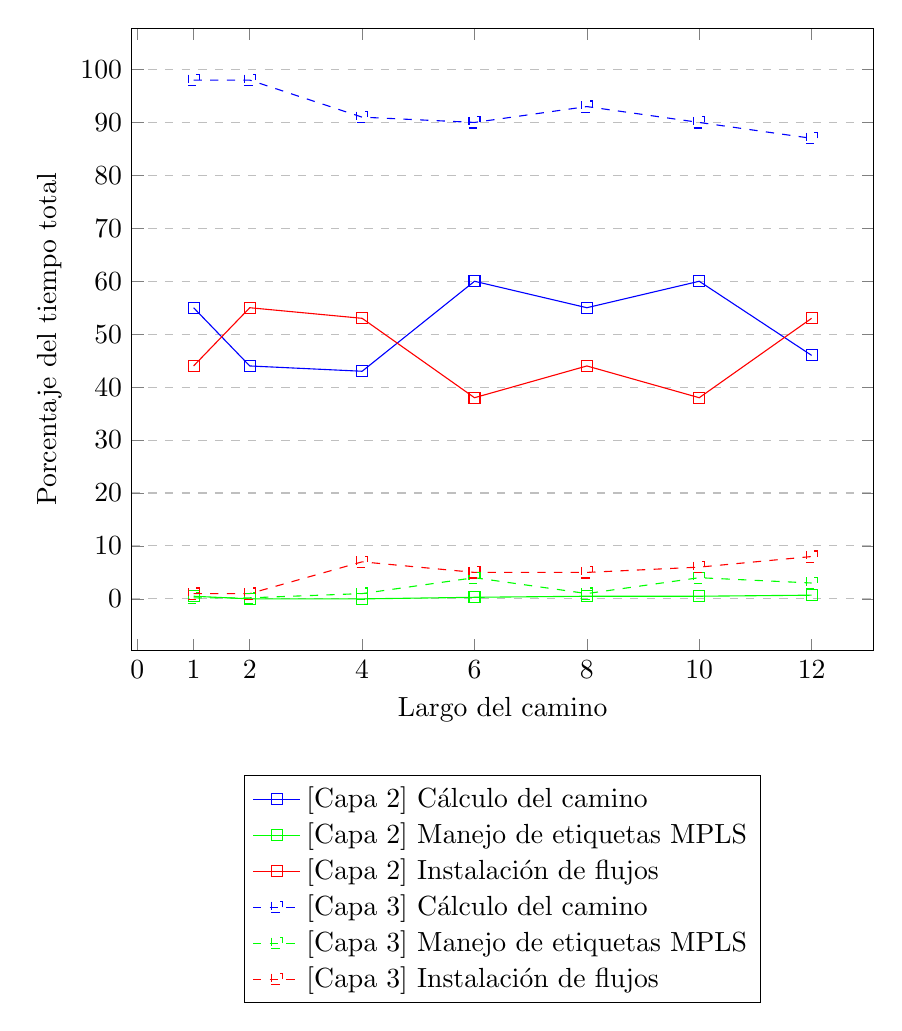
\begin{tikzpicture}
	\begin{axis}[
	xlabel={Largo del camino},
	ylabel={Porcentaje del tiempo total},
	xtick={0,1,2,4,6,8,10,12},
	ytick={0,10,20,30,40,50,60,70,80,90,100},
	scaled x ticks = false,
	x tick label style={/pgf/number format/fixed},
	legend style={at={(0.5,-0.2)},anchor=north},
	ymajorgrids=true,
	grid style=dashed,
	width=11cm,
	legend cell align=left,
	]
	\addplot[
	color=blue,
	mark=square,
	]
	coordinates {
		(1,55)(2,44)(4,43)(6,60)(8,55)(10,60)(12,46)
	};
	\addlegendentry{[Capa 2] Cálculo del camino}
	\addplot[
	color=green,
	mark=square,
	]
	coordinates {
		(1,0.5)(2,0)(4,0)(6,0.3)(8,0.5)(10,0.5)(12,0.7)
	};
	\addlegendentry{[Capa 2] Manejo de etiquetas MPLS}
	\addplot[
	color=red,
	mark=square,
	]
	coordinates {
		(1,44)(2,55)(4,53)(6,38)(8,44)(10,38)(12,53)
	};
	\addlegendentry{[Capa 2] Instalación de flujos}
	\addplot[
	color=blue,
	mark=square,
	dashed,
	]
	coordinates {
		(1,98)(2,98)(4,91)(6,90)(8,93)(10,90)(12,87)
	};
	\addlegendentry{[Capa 3] Cálculo del camino}
	\addplot[
	color=green,
	mark=square,
	dashed,
	]
	coordinates {
		(1,0.2)(2,0.2)(4,1)(6,4)(8,1)(10,4)(12,3)
	};
	\addlegendentry{[Capa 3] Manejo de etiquetas MPLS}
	\addplot[
	color=red,
	mark=square,
	dashed,
	]
	coordinates {
		(1,1)(2,1)(4,7)(6,5)(8,5)(10,6)(12,8)
	};
	\addlegendentry{[Capa 3] Instalación de flujos}
	\end{axis}
	\end{tikzpicture}
\end{figure}

Las líneas rojas muestran como evoluciona el porcentaje del tiempo que abarca la instalación de flujos. Se observa que la porción de tiempo requerida para la instalación de los flujos de una VPN de capa 2 (denotada por las líneas rojas continuas) queda siempre por encima de la requerida para instalar flujos de una VPN de capa 3 (líneas rojas punteadas). Esto se debe a que, como ya fue explicado anteriormente, una VPN de capa 2 debe instalar más flujos en los nodos, lo cual implica que se debe dedicar más tiempo a la etapa de instalación de flujos. Para ambos tipos de VPN se observa que la instalación de flujos abarca más tiempo de ejecución (las líneas suben) a medida que el camino es más largo. Esto es esperable ya que más nodos implican más flujos. Curiosamente, esta suba parece ser más pronunciada para la VPN de capa 3.

Las líneas verdes muestran qué porcentaje del tiempo total se dedica al cálculo y manejo de etiquetas MPLS. Igual que la instalación de flujos, esta etapa requiere más tiempo a medida que hay más nodos en el camino, ya que se aumenta la cantidad de etiquetas MPLS. También se observa que la VPN de capa 3 requiere un mayor porcentaje del tiempo que la de capa 2 para esta tarea. Esto puede resultar extraño, ya que la de capa 2 debe manejar más etiquetas. Lo que ocurre es que la de capa 2 requiere más tiempo absoluto, pero el tiempo total de creación de la VPN también es mayor, por lo tanto el porcentaje del tiempo que se dedica a la tarea resulta mayor para la VPN de capa 3. Otra observación es que esta tarea es la que menos tiempo requiere de las tres.

Por último, el cálculo del camino óptimo. Lo primero a tener en cuenta es que esta etapa no es afectada por el tipo de VPN que se está creando, ya que lo único que debe hacer es determinar el camino óptimo entre dos nodos de un grafo. Tampoco es afectada por el largo del camino que está calculando. Lo único que la afecta es el tamaño de la topología.
Las líneas azules denotan la participación del cálculo del camino óptimo en la distribución del tiempo. Lo primero que se observa es que el porcentaje de tiempo dedicado a esta tarea decrece a medida que se aumenta el largo del camino. Esto es esperable, ya que el tiempo requerido tiende a ser constante, mientras que las otras tareas requieren más tiempo, por lo tanto su porción del tiempo disminuye. Otra observación interesante es que a medida que se aumenta el tamaño de la topología, esta etapa ocupa una mayor parte del tiempo de ejecución. En la topología chica la etapa de instalación de flujos se lleva la mayor parte del tiempo de ejecución tanto para la VPN de capa 2 como la de capa 3. Sin embargo, en la topología mediana eso cambia, y se cumple sólo para la VPN de capa 2. Por último, en la topología grande, ya no se observa eso para ninguno de los dos tipos, y la VPN de capa 2 reparte de forma bastante equitativa el tiempo de ejecución entre el cálculo del camino y la instalación de flujos.

Desde el punto de vista técnico esto también es esperable, ya que el algoritmo que calcula el camino es de orden cuadrático en la cantidad de nodos, mientras que las otras etapas (manejo de etiquetas e instalación de flujos OpenFlow) aumentan linealmente con la cantidad de nodos en el camino. Esto lleva a creer que si se siguiera experimentando con topologias aún más grandes, el cálculo del camino óptimo eventualmente abarcaría la mayoría del tiempo de creación de las VPNs, tanto de capa 2 como de capa 3.


\section{Escala de servicios y flujos}
Entre los requerimientos de la RAU2 se encuentra el de la escalabilidad de usuarios. Específicamente, se espera alcanzar en un mediano plazo un total de 11.000 docentes, 7.000 funcionarios y 140.000 estudiantes (de acuerdo a los requerimientos relevados por el proyecto RRAP). Esto implica que la red será sujeta a importantes cantidades de servicios y flujos distintos. Para poder asegurar que la arquitectura escala sin problemas, se la debería someter a experimentos que reflejen los niveles de actividad y tráfico que son esperados en un futuro. Sin embargo, dichos experimentos no son llevados a cabo por este trabajo por dos razones. En primer lugar, se considera que es una tarea que lleva demasiado tiempo como para ser incluida dentro del alcance de este trabajo. En segundo lugar, no están disponibles los modelos y patrones de tráfico que serían necesarios para esas pruebas.

También es importante recordar que el entorno virtual no generará resultados relevantes en lo que refiere al nivel real de rendimiento de la arquitectura. Recordar sección 3.3.1, donde se explica que cada instancia de Open vSwitch se ejecuta en modo user-space, y por ende procesa los paquetes de forma bastante lenta.

Se puede concluir entonces que las pruebas detalladas a continuación no aseguran la escalabilidad de RAUFlow, pero sí ayudan a investigar el comportamiento de la red y los dispositivos cuando se los somete a muchos servicios.

\subsection{Descripción del escenario}
El escenario de prueba consiste en crear una cantidad relativamente grande de VPNs en la topología básica, y analizar si esto degrada el rendimiento de la red de alguna forma. Se utiliza una VPN punto a punto de capa 3 para conectar dos subredes cliente, y se utiliza \textit{iperf} para generar tráfico TCP y medir el ancho de banda entre los dos hosts. Para cargar al controlador con servicios, se crean múltiples VPN de capa 2 entre las subredes, variando los valores de los cabezales VLAN\_ID y VLAN\_PCP (pudiendo crear un total de 32.768 combinaciones distintas) para que toda VPN sea distinta de las demás. De esta forma, existirán múltiples VPN pero solo una (la de capa 3) será utilizada con tráfico. \\
Dado que cargar todas las VPN a mano en la interfaz web llevaría demasiado tiempo, se creó un servicio web que recibe como parámetro la cantidad de VPN que se desean. Cuando se hace un pedido GET a ese servicio web, se inicia el proceso de creación de las mismas. Este proceso puede tomar entre algunos minutos y varias horas, dependiendo de la cantidad. \\ \\
Con este escenario de prueba se busca verificar los dos siguientes aspectos claves: \\ \\
\textbf{Escalabilidad interna del RAUSwitch} \\
Se estudian posibles limitaciones internas que puedan tener los dispositivos cuando deben manejar grandes cantidades de flujos. Es posible que a medida que crecen sus tablas de flujos, demoren más en encontrar el flujo que se corresponde con cada paquete que reciben. Si pasa esto, el throughput debería ser afectado negativamente por la cantidad de flujos en sus tablas.
\textbf{Escalabilidad en servicios} \\
Se estudian posibles problemas que puedan tener la arquitectura de la red o, en particular, la aplicación RAUFlow para manejar grandes cantidades de servicios o información. Es de particular interés medir la memoria que requiere el controlador para mantener los servicios. \\ \\

\subsection{Resultados y observaciones}

\begin{table}[ht]
	\caption{Throughput en Kbits/s medidos para distintas cantidades de VPNs.}
	\centering 
	\begin{tabular}{c c}
		\hline\hline
		\# de VPNs & Throughput (Kbits/s) \\ [0.5ex]
		\hline
		1 & 893 \\
		3000 & 887 \\
		6000 & 887 \\
		9000 & 890 \\
		12000 & 885 \\
		15000 & 886 \\ [1ex]
		\hline
	\end{tabular}
	\label{table:escala_de_servicios}
\end{table}

Como se explica en la descripción del escenario, se busca determinar si la existencia de muchos flujos en la tabla implica que un RAUSwitch demora más tiempo en encontrar el flujo OpenFlow que corresponde para un paquete entrante, y por lo tanto demora más en determinar la acción a tomar para ese paquete. Si esto fuera así, debería existir una relación inversamente proporcional entre la cantidad de flujos en la tabla de un nodo y su velocidad para procesar paquetes. En la tabla \ref{table:escala_de_servicios} se pueden observar los throughput promedio medidos para un flujo de datos sobre la topología básica, con distintas cantidades de VPN existiendo en la red. La principal conclusión que se puede sacar de la tabla es que el throughput no es afectado por la cantidad de VPNs existentes en el momento (se asume que las pequeñas diferencias numéricas entran en el margen de error).

Se puede ver que la máxima cantidad de VPNs con la que se probó fue de 15.000. Cada VPN de capa 2 está compuesta por dos servicios de capa 2, y cada uno de esos servicios introduce 42 flujos en cada nodo del camino. Esto quiere decir que cada uno contiene alrededor de 1.260.000 (15.000 * 2 * 42) flujos en su tabla. Se podría argumentar que hacen falta más flujos para impactar el throughput, pero en realidad la explicación se encuentra en la especificación de Open vSwitch, y ya fue mencionada en el capítulo 3. Open vSwitch realiza cacheo de flujos. Eso quiere decir que cuando un paquete de datos de un determinado flujo llega por primera vez a un nodo, este paquete es enviado al pipeline de OpenFlow para determinar qué acción se debe tomar. Luego de realizada, esta acción es escrita en la caché, y tiene un tiempo de vida de entre 5 y 10 segundos. Si en ese período de tiempo llega otro paquete del mismo flujo, no hay necesidad de enviar el paquete al pipeline, porque ya se sabe cuales son las acciones a tomar para el mismo. Por lo tanto, si un flujo de datos es constante y rápido, el tamaño de la tabla de OpenFlow no afectará el tiempo de decisión, ya que sólo el primer paquete de ese flujo deberá ser comparado con dicha tabla.

Mediante el comando 'ovs-appctl dpctl/show' de Open vSwitch, se puede examinar las estadísticas de la cache de cada nodo. A modo de ejemplo, en la figura \ref{fig:cache_sample} se observan las estadísticas de un nodo llamado 'alice'. En la sección 'lookups' se detallan cuantos 'hits' y 'miss' de caché han ocurrido hasta el momento, y 'flows' indica cuantos flujos activos hay en el momento en la caché.

\begin{figure}[H]
	\caption{Estadísticas de cache de flujos del nodo 'alice'.}
	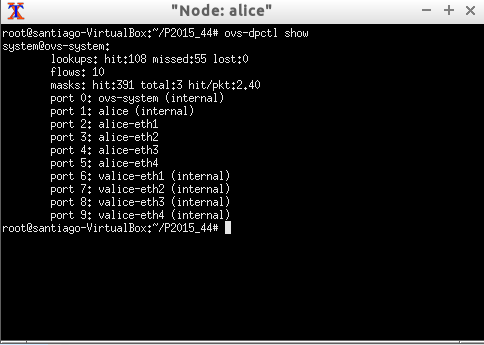
\includegraphics[scale=1]{cache_sample}
	\centering
	\label{fig:cache_sample}
\end{figure}

Otro objetivo de la prueba es determinar si la arquitectura, y en particular el controlador, tienen algún problema para manejar muchos servicios. No se ha detectado ningún problema de esa índole. Sin embargo, es importante recordar que el controlador mantiene toda su información en memoria, por lo tanto es de interés realizar un estudio del consumo de memoria del mismo a medida que crece la cantidad de servicios. El comando de Linux llamado \textit{pmap} permite estudiar el consumo de memoria del proceso que se le indique, y con el mismo se puede analizar la evolución del consumo de memoria del controlador a medida que se le agregan servicios. En la tabla \ref{table:consumo_de_memoria} y la figura \ref{fig:consumo_de_memoria} se puede observar el resultado de estas mediciones. \\

\begin{table}[ht]
	\caption{Evolución del consumo de memoria del controlador.}
	\centering 
	\begin{tabular}{c c}
		\hline\hline
		\# de VPNs & Memoria (KB) \\ [0.5ex]
		\hline
		0 & 33280 \\
		3000 & 108196 \\
		6000 & 182460 \\
		9000 & 256528 \\
		12000 & 333244 \\
		15000 & 407696 \\ [1ex]
		\hline
	\end{tabular}
	\label{table:consumo_de_memoria}
\end{table}

\begin{figure}
\caption{Efecto de la cantidad de VPN sobre la memoria consumida}
\centering
\label{fig:consumo_de_memoria}
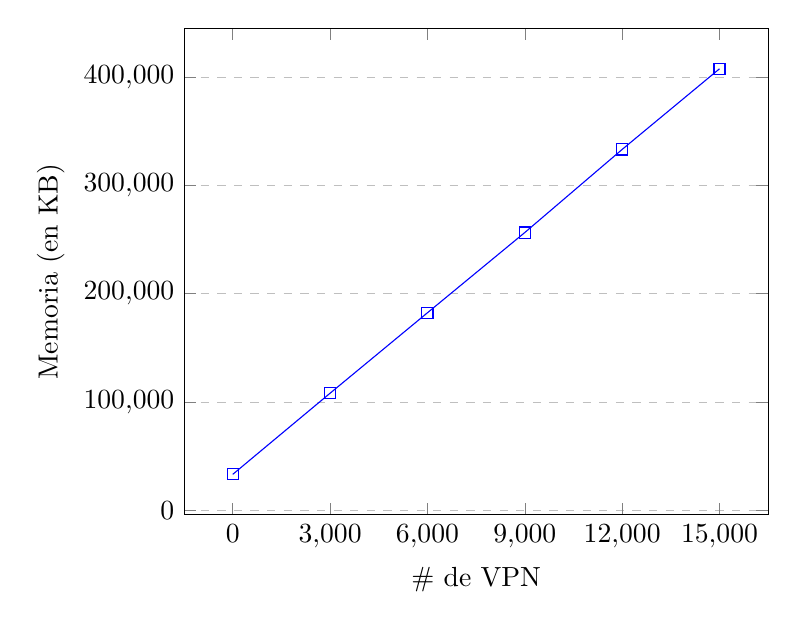
\begin{tikzpicture}
\begin{axis}[
xlabel={\# de VPN},
ylabel={Memoria (en KB)},
xtick={0,3000,6000,9000,12000,15000},
ytick={0,100000,200000,300000,400000,500000},
scaled x ticks = false,
scaled y ticks = false,
x tick label style={/pgf/number format/fixed},
y tick label style={/pgf/number format/fixed},
legend pos=north west,
ymajorgrids=true,
grid style=dashed,
]
\addplot[
color=blue,
mark=square,
]
coordinates {
	(0,33280)(3000,108196)(6000,182460)(9000,256528)(12000,333244)(15000,407696)
};
\end{axis}
\end{tikzpicture}
\end{figure}

La principal observación que se puede hacer es que el consumo de memoria del controlador aumenta de forma lineal con la cantidad de servicios. El mismo se incrementa en 74916 KB cada 3000 servicios, por lo tanto se puede calcular que cada servicio ocupa alrededor de 25 KB (74916/3000). A modo de ejemplo, si extrapolamos ese número a una computadora que puede dedicar 4 Gb de RAM para mantener los servicios, llegamos a que el controlador podrá mantener alrededor de 167.772 servicios. A pesar de que no es ideal mantener tantos datos en memoria, se puede concluir que es un consumo aceptable. \\

En el proceso de realizar las pruebas ya mencionadas también se observó un comportamiento que no se esperaba. Se detectó que a medida que hay más VPNs creadas, la red demora más tiempo en crear una nueva VPN. Con el propósito de entender más ese comportamiento, se hizo un experimento cuyos resultados se observan en la figura \ref{fig:tiempo_vpns_acumuladas}.

\begin{figure}
\caption{Efecto de la cantidad de VPNs sobre el tiempo de carga de una VPN nueva}
\centering
\label{fig:tiempo_vpns_acumuladas}
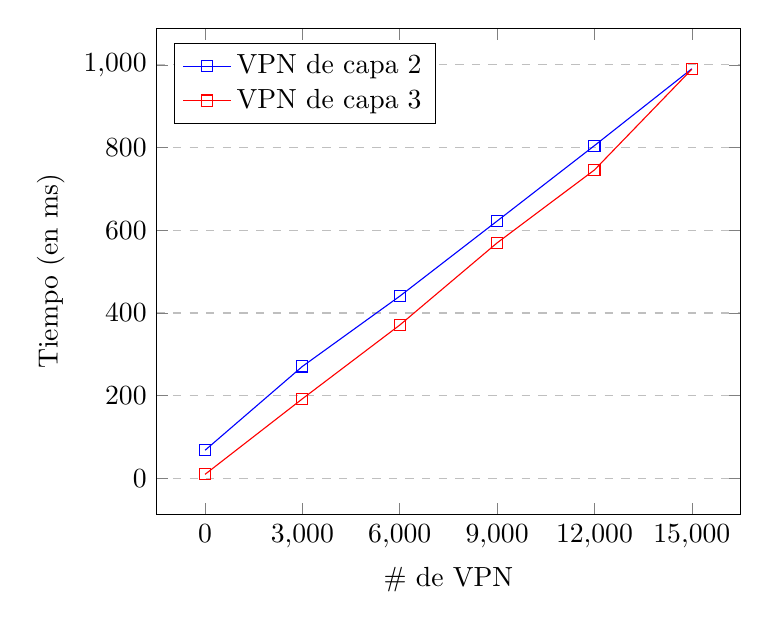
\begin{tikzpicture}
\begin{axis}[
xlabel={\# de VPN},
ylabel={Tiempo (en ms)},
xtick={0,3000,6000,9000,12000,15000},
ytick={0,200,400,600,800,1000,1200},
scaled x ticks = false,
x tick label style={/pgf/number format/fixed},
legend pos=north west,
ymajorgrids=true,
grid style=dashed,
]
\addplot[
color=blue,
mark=square,
]
coordinates {
	(1,68.2)(3000,270.9)(6000,440.7)(9000,622.4)(12000,804.8)(15000,990.5)
};
\addlegendentry{VPN de capa 2}
\addplot[
color=red,
mark=square,
]
coordinates {
	(1,10.0)(3000,192.6)(6000,370.9)(9000,569.6)(12000,746.0)(15000,989.3)
};
\addlegendentry{VPN de capa 3}
\end{axis}
\end{tikzpicture}
\end{figure}

Cada punto indica el tiempo que demora la red en dar de alta una nueva VPN con una determinada cantidad de VPN ya existentes. Estos tiempos se miden de la misma forma que los obtenidos en la sección de pruebas anterior: se toma el tiempo que demora la aplicación en devolver la respuesta HTTP indicando que el servicio se creó con éxito (disponible en los logs). En la gráfica se puede ver que el tiempo de carga aumenta de forma lineal a medida que hay más VPN en la red, y esto se cumple para la de capa 2 como la de capa 3. Una posible explicación inicial para esto puede ser que al tener más flujos, cada nodo demora más en insertar nuevos flujos en su tabla. Esa teoría se descarta con el siguiente razonamiento. En la gráfica se observa que toma más tiempo crear una VPN de capa 2 que una de capa 3. Esto en gran medida se explica porque un servicio de capa 2 debe insertar 42 flujos en los nodos del camino, mientras que uno de capa 3 solo inserta 1. Pero también se observa que las lineas son virtualmente paralelas, es decir, esa diferencia de tiempo se mantiene constante a pesar de las VPNs que existan. Si insertar un flujo nuevo cada vez tomara más tiempo, ese incremento se debería multiplicar por 42 para la VPN de capa 2, y la linea correspondiente a la VPN de capa 2 debería tener una pendiente más inclinada que la de capa 3.

Otra posible explicación para este comportamiento, y quizás la más probable, es que la aplicación RAUFlow se vuelve más lenta a medida que sus estructuras de datos crecen. Sin embargo, no se observa ninguna característica en el código que indique esto.

\chapter{Conclusiones}

% **************************** Define Graphics Path **************************
\graphicspath{{Chapter5/Figs/}}

Se realizó una investigación del estado del arte de las diferentes aplicaciones que se le puede dar al paradigma SDN, prestando especial atención a las diferentes maneras de implementar redes privadas virtuales. También se hizo una investigación profunda sobre las diferentes opciones de virtualización para las redes definidas por software.

Tomando como base al popular emulador Mininet, se construyó una herramienta que permite emular dispositivos que pueden actuar como switches OpenFlow y al mismo tiempo correr protocolos distribuidos legados como OSPF. Esta herramienta permite la virtualización de la arquitectura RAUFlow, pero también se la puede ver como un resultado valioso incluso afuera del contexto de RAUFlow, ya que hasta el momento de realizar este trabajo no se encontró ninguna herramienta que tenga esas capacidades. Se creó un repositorio público en Github \cite{gitp2015_44} con el código fuente del emulador con la intención de hacerlo disponible para la comunidad. También se produjo un manual de usuario para facilitar el uso futuro de la herramienta.

Se trabajó en una verificación funcional del entorno construido, que permitió detectar y corregir problemas, y validar el correcto funcionamiento del mismo con diversas topologias. Dicha verificación también permitió corregir dos defectos en el código fuente de la aplicación RAUFlow, y detectar algunos posibles problemas de escalabilidad de la arquitectura. También se implementó una mejora a RAUFlow, que permite eliminar la necesidad de agentes SNMP en cada RAUSwitch, reduciendo la complejidad y posiblemente aumentando el rendimiento de los mismos.

Usando la herramienta construida se realizó una serie de pruebas para estudiar la escalabilidad de RAUFlow. En primer lugar, mediante diferentes topologias de prueba se estudió el tiempo requerido para la creación de VPNs. Para profundizar el análisis, se estudió la distribución del tiempo de ejecución entre las principales tareas que componen dicho proceso de creación. En segundo lugar, se llevó a cabo una serie de pruebas que estudian el comportamiento de RAUFlow y los RAUSwitch cuando existen muchos servicios. Desde el punto de vista de los RAUSwitch, un estudio a fondo de la herramienta Open vSwitch determinó que la existencia de muchos servicios no afecta el rendimiento de los mismos. Desde el punto de vista del controlador, se verificó que no tiene problemas para mantener muchos servicios, y se estudió la evolución de su consumo de memoria.

Por último, este trabajo contribuyó a la realización de una publicación científica llamada "RAUflow: building Virtual Private Networks with MPLS and OpenFlow" \cite{rauflow}, la cual fue presentada recientemente en la conferencia ACM SIGCOMM Workshop on Fostering Latin-American Research in Data Communication Networks (LANCOMM 2016).

%mencionar SSN si corresponde

\section{Trabajo futuro}

Si bien en este trabajo se ha desarrollado un emulador completamente funcional, aún existe lugar para mejorarlo. Por ejemplo, la configuración de nuevas topologias se debe hacer mediante scripts en Python. Si bien la API para hacerlo es relativamente simple, la tarea puede ser tediosa si se trata de topologias grandes. Existe una propuesta de interfaz gráfica para Mininet llamada MiniEdit \cite{miniedit} que puede ser utilizada con el propósito de mejorar la usabilidad del entorno virtual. Es probable que sea necesario modificar MiniEdit para que funcione con el entorno construido, pero esto no debería ser una tarea muy compleja ya que el código fuente está disponible y bien documentado.

El entorno construido también puede ser mejorado para proporcionar experimentos más reales, o fieles a la realidad. Existe una extensión de Mininet llamada Mininet-HiFi \cite{mininet-hifi} que apunta a mejorar Mininet para proveer experimentos más realistas y reproducibles. Utiliza conceptos como límites de CPU, control de tráfico y aislamiento de recursos para intentar que el experimento que se lleve a cabo sea lo más fiel posible al mismo escenario pero con hardware real.
Otra posible línea de trabajo con el objetivo de aumentar el realismo de los experimentos es investigar la herramienta Open vSwitch para encontrar maneras de hacer que múltiples switches OpenFlow en distintos network namespaces puedan procesar paquetes a nivel del kernel. Esto aumentaría sustancialmente la velocidad de los switches que ofrece el entorno virtual actualmente, y ayudaría a que los switches emulados se asemejen más a los físicos.

Se han hecho diversas pruebas sobre la arquitectura RAUFlow que muestran que posee una buena escalabilidad. Sin embargo, es necesario hacer más pruebas para poder asegurarlo. Desde el punto de vista de la escalabilidad en las topologias, en la sección 3.5 se detallaron algunos problemas funcionales que se sospecha pueden afectar un despliegue real de la arquitectura, y por ende se sugiere una investigación a fondo sobre los mismos. Desde el punto de vista de la escalabilidad en el uso, no se hicieron pruebas con modelos de tráfico que reflejen el volumen y características del tráfico que se espera en la red. Esto es un paso clave en la determinación de la escalabilidad de RAUFlow.

Sería interesante implementar nuevas funcionalidades sobre la arquitectura RAUFlow que incorporen nociones como Ingeniería de tráfico, Quality of Service y seguridad de la red.

Se ha mencionado que el controlador de RAUFlow almacena todos sus datos en memoria. Implementar un método de persistencia que no dependa de la memoria del sistema podría mejorar la escalabilidad y también la robustez, ya que el controlador se podría recuperar ante fallas.

También se discutió que mantener comunicación con demasiados switches OpenFlow puede ser un problema para el controlador, lo cual presentaría un serio problema de escalabilidad. La existencia de un único centro de cómputo para el control de la red también puede generar un efecto cuello de botella. Estos problemas pueden ser solucionados utilizando múltiples controladores, y estableciendo una relación de jerarquía entre ellos.

%\include{Chapter6/chapter6}
%\include{Chapter7/chapter7}



% ********************************** Back Matter *******************************
% Backmatter should be commented out, if you are using appendices after References
%\backmatter

% ********************************** Bibliography ******************************
\begin{spacing}{0.9}

% To use the conventional natbib style referencing
% Bibliography style previews: http://nodonn.tipido.net/bibstyle.php
% Reference styles: http://sites.stat.psu.edu/~surajit/present/bib.htm

\bibliographystyle{apalike}
%\bibliographystyle{unsrt} % Use for unsorted references  
%\bibliographystyle{plainnat} % use this to have URLs listed in References
\cleardoublepage
\nocite{*}
\bibliography{References/references} % Path to your References.bib file


% If you would like to use BibLaTeX for your references, pass `custombib' as
% an option in the document class. The location of 'reference.bib' should be
% specified in the preamble.tex file in the custombib section.
% Comment out the lines related to natbib above and uncomment the following line.

%\printbibliography[heading=bibintoc, title={References}]


\end{spacing}

% ********************************** Appendices ********************************

\begin{appendices} % Using appendices environment for more functunality

% ******************************* Thesis Appendix A ****************************

\graphicspath{{Appendix1/Figs/}}

\chapter{Manual de usuario del emulador}

\section{Modo de uso}
Para utilizar el emulador es necesario instalar:
\begin{itemize}
	\item Mininet. Version 2.2.1 o mayor.
	\item Open vSwitch. Version 2.4.0 o mayor.
	\item Quagga. Probado con versión 0.99.22.4-3ubuntu1.
\end{itemize}

Posicionándose en el directorio raíz del proyecto, iniciar el emulador con el siguiente comando:
\begin{lstlisting}
sudo python start.py {RUTA_TOPOLOGIA}
\end{lstlisting}

El valor de \{RUTA\_TOPOLOGIA\} debe ser el path hacia el script Python que configura la topología. Para conocer los detalles de lo que debe hacer ese script, leer la sección A.2.

El script \textbf{start.py} realiza las siguientes funciones:
\begin{itemize}
	\item Carga la topología recibida por parámetro y la inicia.
	\item Borra el archivo utils/init\_json.json, en caso de que una ejecución previa lo haya creado. El propósito de este archivo se verá mas adelante.
	\item Llama al método \textbf{start} de cada nodo virtual. Cada una de las cuatro clases de nodos (RAUSwitch, RAUHost, RAUController y QuaggaRouter) tiene este método, que se encarga de inicializar y configurar el nodo.
\end{itemize}

Luego de iniciar, Mininet ofrece una línea de comandos con la que el usuario puede interactuar. Ejecutando el siguiente comando se puede obtener una terminal Linux en cualquiera de los nodos.
\begin{lstlisting}
xterm {NOMBRE_NODO}
\end{lstlisting}

De aquí en adelante en este manual de usuario, cuando se indique que hay que ejecutar un determinado comando en un nodo, se lo debe ejecutar en una consola xterm en dicho nodo.

Habiendo iniciado el entorno virtual, hay que llevar a cabo algunos pasos más para que sea totalmente funcional:
\begin{enumerate}
	\item Esperar a que OSPF termine de distribuir las rutas y actualizar las bases de datos topológicas. Este proceso en general toma menos de un minuto, y varía de acuerdo al tamaño de la topología. Una manera de verificar esto es con el comando \textbf{route} y analizando la tabla de ruteo de los nodos.
	\item Ejecutar el comando \textbf{python telnetRouters.py} desde el nodo controlador o desde cualquier RAUSwitch. Este script Python es el que se invocaría automáticamente si se detectara un cambio en la topología (en el entorno virtual se lo llama manualmente) y se encarga de consultar la base de datos topológica de OSPF mediante Telnet, parsear la información y enviarla a la aplicación RAUFlow. Es importante asegurarse que el paso 1 esté completo antes de ejecutarlo, ya que en caso contrario la base de datos de OSPF estará incompleta y se estarán enviando datos incorrectos. Luego de recibir la topología, la aplicación RAUFlow todavía necesita la siguiente información de cada RAUSwitch: nombres de interfaces, direcciones IP y direcciones MAC. Para obtener esta información, se conecta automáticamente con el nodo que tiene levantado el Web Service que hace disponible la información de cada nodo. En la versión del código que se entrega, el nodo que levanta el Web Service es el controlador mismo (es decir, se conecta consigo mismo mediante localhost) pero puede ser cualquiera, siempre y cuando esté ejecutando el script \textbf{utils/wsOVS.py}. Este script es el sustituto que se creó para suplantar a \textbf{wsSNMP.py} (recordar sección 3.3.5).
	\item Para poder crear servicios en RAUFlow, se debe indicar cuales RAUSwitch son de borde y cuales no. En el caso de los que son de borde, también se debe especificar la dirección IP y MAC del nodo CE (que típicamente será un RAUHost o QuaggaRouter) con el que el RAUSwitch está conectado. Tradicionalmente esto se hace en la interfaz web de RAUFlow, pero esto resulta tedioso y lento si se tienen muchos nodos. Para acelerar este proceso se creó un script llamado \textbf{nodeInits.py} que se puede ejecutar desde cualquier nodo, y se encarga de enviar toda esa información al controlador mediante pedidos HTTP. La ejecución de este script es opcional; si el usuario desea puede ingresar los datos mediante la interfaz web. El script envía los datos que se encuentren en el archivo \textbf{init\_json.json}, y dicho archivo es creado automáticamente cuando se levanta el emulador. En caso de hacerse, la ejecución de este script debe ser posterior a la de telnetRouters.py, ya que en caso contrario se estarían mandando datos de nodos que el controlador todavía no conoce. En la sección A.2 se explicará como indicarle al emulador que nodos son de borde, así como las direcciones de los nodos CE.
\end{enumerate}

Luego de que el entorno está levantado y listo para usarse, se puede empezar a crear servicios. Para usar la interfaz web de RAUFlow se debe levantar un explorador desde el nodo controlador. Esto se puede lograr primero iniciando una consola xterm en dicho nodo, y luego ejecutando el comando que inicie el explorador (por ejemplo, \textbf{firefox}). Una vez en la interfaz web de RAUFlow, se puede interactuar con ella de forma normal.

Al agregar VPNs, es importante tener en cuenta que las rutas de los nodos clientes involucrados deben estar correctamente configuradas, ya sea tratándose de una VPN de capa 2 o 3. En el caso de la VPN de capa 3, los nodos CE involucrados en la VPN deben tener como gateway al RAUSwitch de borde correspondiente. Esto se puede lograr con el comando \textbf{route} tradicional de Linux o mediante el uso del parámetro \textbf{gw} al configurar la topología. En la VPN de capa 2, los nodos CE involucrados deben tener sus rutas configuradas de tal forma para que actúen como si estuvieran directamente conectados.

Para crear una VPN, recordar que se deben crear dos servicios: uno para el tráfico de ida y uno para el de vuelta. Para crear una VPN de capa 2 alcanza con indicar los nodos de entrada y salida, y no es necesario indicar ethertype ya que al ser de capa 2 permitirá todo tipo de tráfico. En el caso de una VPN de capa 3, se debe además indicar el ethertype correspondiente (por ejemplo, para tráfico IP sería 0x0800).

\section{Cómo interactuar con cada instancia de Open vSwitch}
Como se explica en el capítulo 3, cada RAUSwitch tiene su propia instancia de Open vSwitch ejecutándose en modo userspace. Esto modifica un poco la manera de usar sus comandos, ya que cada comando se debe "apuntar" a la instancia con la que se desea interactuar.

Cada RAUSwitch tiene un directorio bajo /tmp donde se almacenan los archivos relacionados con su instancia de Open vSwitch y Quagga. El siguiente diagrama explica la estructura de archivos correspondiente a un nodo llamado "switch1". 
\dirtree{%
	.1 /.
	.2 tmp.
	.3 switch1.
	.4 ovs.
	.5 db.sock.
	.5 ovs-vswitchd.ctl.
	.4 quagga.
}

El diagrama muestra dos archivos que son vitales para poder comunicarse con la instancia de Open vSwitch del nodo "switch1". Estos son: \textbf{db.sock} y \textbf{ovs-vswitchd.ctl}. El propósito de estos archivos se explicará más adelante. Los demás archivos que se mantienen en estos directorios son los relacionados con Quagga, y se omiten por simplicidad.

Open vSwitch tiene varias herramientas que permiten consultar datos y realizar configuraciones. Las de interés en este contexto son: ovs-appctl, ovs-vsctl, ovs-ofctl y ovs-dpctl. A continuación se explicará en que consiste cada una y como usarla apuntando a un nodo específico.
\begin{itemize}
	\item \textbf{ovs-appctl} \cite{ovs-appctl} es una herramienta que permite enviarle comandos al demonio ovs-vswitchd. Se le puede consultar cosas como flujos, logs, etc, así como realizar configuraciones en tiempo de ejecución. El entorno virtual tendrá múltiples instancias de este demonio ejecutando, así que es necesario indicar a qué instancia debe ser dirigido un comando. Esto se hace con la opción \textbf{-t} o \textbf{--target} seguido por el socket de Unix en el cual la instancia está escuchando por conexiones de control. Aquí entra en juego el archivo \textbf{ovs-vswitchd.ctl} mencionado anteriormente. Al iniciarse, cada instancia de Open vSwitch almacenará ese socket en el directorio privado de su nodo. Por lo tanto, para apuntar un comando "ovs-appctl" hacia un nodo específico se debe hacer: \textit{ovs-appctl --target=/tmp/nombre\_nodo/ovs/ovs-vswitchd.ctl nombre\_comando}.
	\item \textbf{ovs-vsctl} \cite{ovs-vsctl} permite conectarse con el proceso ovsdb-server, quien se encarga de mantener la base de datos de configuración de Open vSwitch. ovs-vsctl permite consultar y modificar dicha base de datos. Igual que en el caso de ovs-appctl, se debe especificar a que instancia se desea apuntar el comando. Esto se logra con la opción \textbf{--db}, que indica el modo de conexión que se utilizará. Este puede ser: un socket de Unix o la red. En caso de usar un socket de Unix, se debe indicar la ruta al archivo \textbf{db.sock} que le corresponde al nodo, de la siguiente manera: \textit{ovs-vsctl --db=unix:/tmp/nombre\_nodo/ovs/db.sock nombre\_comando}. Por otro lado, si se desea enviar el comando a través de la red, se debe ejecutar: \textit{ovs-vsctl --db=tcp:dirección\_ip:6640 nombre\_comando} usando la dirección IP del nodo de interés.
	\item \textbf{ovs-ofctl} \cite{ovs-ofctl} permite monitorear y administrar el switch OpenFlow. Por ejemplo, un uso frecuente es el de consultar el contenido de las tablas de flujos de un switch, que se hace con el siguiente comando: \textit{ovs-ofctl -O OpenFlow13 dump-flows nombre\_nodo}. A diferencia de las herramientas anteriores, no hace falta indicar de una forma especial a qué nodo apunta el comando. Alcanza con ejecutarlo en una consola xterm en el nodo que se busca administrar.
	\item \textbf{ovs-dpctl} \cite{ovs-dpctl} es un programa que permite consultar y administrar los flujos de los datapaths externos a ovs-vswitchd, como el datapath del kernel. El datapath del kernel no es utilizado en el entorno (debido a las múltiples instancias de Open vSwitch), por lo tanto no es posible usar esta herramienta. Para administrar el datapath en el userspace (también llamado netdev) se puede utilizar la familia de comandos \textit{dpctl/*} de ovs-appctl. Por ejemplo, \textit{ovs-appctl  --target=/tmp/nombre\_nodo/ovs/ovs-vswitchd.ctl dpctl/show} muestra las estadísticas del cache de flujos para un determinado nodo.
\end{itemize}

\section{API para configurar las topologias}
La API que se debe usar para crear y personalizar las topologias es, en esencia, la misma que la de Mininet estándar. Cada topología debe ser configurada por un script Python, que debe definir una subclase de la clase \textit{Topo} de Mininet. A dicha subclase se le debe agregar nodos y enlaces mediante los métodos \textit{addHost}, \textit{addSwitch}, y \textit{addLink}. En el caso de los dos primeros, es necesario indicar la clase de nodo que se está agregando, y los parámetros necesarios para inicializar esa clase. Como se explica en el capítulo 3, se crearon cuatro nuevas clases de nodos, y a continuación se detallan los parámetros que se pueden usar en sus constructores. Los resaltados con * son obligatorios. \\

\underline{RAUSwitch}
\begin{itemize}
	\item \textbf{nombre} \textcolor{red}{*}. Nombre del switch.
	\item \textbf{ips} \textcolor{red}{*}. Lista con todas las direcciones IP (en formato CIDR, A.B.C.D/E) para el switch.
	\item \textbf{dpid} \textcolor{red}{*}. Datapath ID del switch. Debe ser un string hexadecimal de largo 16. En caso de no proveer este valor, el datapath ID se derivará del nombre del switch. Por ejemplo: si el nombre es \textit{switch8}, su datapath ID será 8.
	\item \textbf{controller\_ip} \textcolor{red}{*}. Dirección IP del controlador.
	\item \textbf{border}. Número entre 0 o 1 que indica si el switch es de borde o no. Si no se provee, se asume que border=0.
	\item \textbf{ce\_ip\_address}. Dirección IP del nodo CE con el que está conectado. Solo aplica si el switch es de borde.
	\item \textbf{ce\_mac\_address}. Dirección MAC del nodo CE con el que está conectado. Solo aplica si el switch es de borde.
\end{itemize}

\underline{RAUHost}

\begin{itemize}
	\item \textbf{nombre} \textcolor{red}{*}. Nombre del host.
	\item \textbf{ips} \textcolor{red}{*}. Lista con todas las direcciones IP (en formato CIDR, A.B.C.D/E) para el host. En general tendrá una única dirección IP, pero por si acaso se permite que tenga varias.
	\item \textbf{gw}.  Dirección IP del default gateway. Es útil para el uso de VPN de capa 3.
	\item \textbf{ce\_mac\_address}. En caso de que el host se esté usando como nodo CE, este parámetro indica la dirección MAC que debe tener la interfaz que lo conecta con el RAUSwitch. En caso de existir, dicha interfaz debe ser la menor de todas.
\end{itemize}

\underline{RAUController}

\begin{itemize}
	\item \textbf{nombre} \textcolor{red}{*}. Nombre del controlador.
	\item \textbf{ips} \textcolor{red}{*}. Lista con todas las direcciones IP (en formato CIDR, A.B.C.D/E) para el controlador. En general tendrá una única dirección IP, pero por si acaso se permite que tenga varias.
\end{itemize}

\underline{QuaggaRouter}

\begin{itemize}
	\item \textbf{nombre} \textcolor{red}{*}. Nombre del router.
	\item \textbf{ips} \textcolor{red}{*}. Lista con todas las direcciones IP (en formato CIDR, A.B.C.D/E) para el router.
	\item \textbf{gw}.  Dirección IP del default gateway. Es útil para el uso de VPN de capa 3.
	\item \textbf{ce\_mac\_address}. En caso de que el router se esté usando como nodo CE, este parámetro indica la dirección MAC que debe tener la interfaz que lo conecta con el RAUSwitch. En caso de existir, dicha interfaz debe ser la menor de todas.
\end{itemize}

Cada nodo tendrá un conjunto de interfaces de red, definidas de acuerdo a como se creen los enlaces de ese nodo. Por ejemplo, el siguiente fragmento de código crea enlaces entre tres nodos llamados \textit{switch1}, \textit{switch2} y \textit{switch3}:
\begin{lstlisting}
addLink(switch1, switch2, 0, 0)
addLink(switch1, switch3, 1, 0)
\end{lstlisting}

Los últimos dos parámetros indican qué número de interfaz debe tener cada nodo. La primera línea significa que tanto el switch1 como el switch2 tendrán eth0 conectadas a ese enlace. La segunda indica que el switch1 usará eth1 para el enlace, mientras que el switch3 usará eth0. Es importante prestar especial atención a esto, ya que el parámetro \textit{ips} con el que se inicializa cada nodo debe cumplir ciertas reglas:
\begin{itemize}
	\item La cantidad de direcciones IP debe coincidir con la cantidad de interfaces de red.
	\item Las direcciones IP serán asignadas según el orden en el que están en la lista, empezando desde la interfaz más baja.
	\item Si se trata de un RAUSwitch, la primera interfaz (y por ende la primera dirección IP de la lista) debe ser la de la red de gestión.
	\item Si se trata de un RAUSwitch y es de borde, la última interfaz debe ser la que lo conecte con el nodo CE, ya sea un RAUHost o un QuaggaRouter.
	\item Si se trata de un RAUHost o QuaggaRouter que actúa como nodo CE (es decir, está conectado a un RAUSwitch), la primera interfaz debe ser la que lo conecte con el RAUSwitch.
\end{itemize}

Estas restricciones son necesarias dado que el código que inicializa los nodos debe poder distinguir los distintos tipos de interfaces (red de gestión, red interna, customer edge). Una posible alternativa sería que el usuario cree las interfaces sin ningún tipo de restricción de orden, y con parámetros adicionales indique, para cada nodo, el tipo de cada interfaz. Se opta entonces por la solución que evita el uso de más parámetros, pero deja a cargo del usuario asegurarse que se cumplen las reglas establecidas.

\subsection{Ejemplo}
\begin{figure}[t]
	\caption{Topología de ejemplo}
	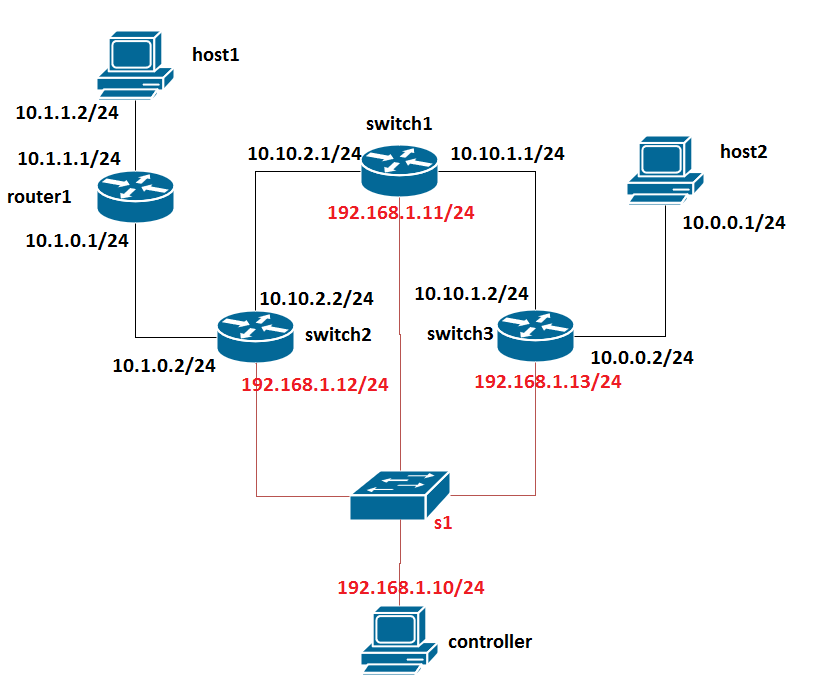
\includegraphics[width=\textwidth,height=\textheight,keepaspectratio]{topo-ejemplo}
	\centering
	\label{fig:topo_ejemplo}
\end{figure}

En la figura \ref{fig:topo_ejemplo} se puede ver una pequeña topología de ejemplo que consiste de 3 RAUSwitch, 1 QuaggaRouter actuando como CE, un RAUHost actuando como CE y otro RAUHost conectado al QuaggaRouter. También se puede ver la red de gestión marcada con rojo. A continuación se muestra el código que implementa esa topología:

\begin{minted}[fontsize=\scriptsize]{python}
from mininet.topo import Topo
from rau_nodes import RAUSwitch, QuaggaRouter, RAUController, RAUHost

class CustomTopology( Topo ):
  def __init__( self ):
	Topo.__init__( self )

	# Hosts
	host1 = self.addHost('host1',
		ips=['10.1.1.2/24'],
		cls=RAUHost)
	host2 = self.addHost('host2',
		ips=['10.0.0.1/24'],
		ce_mac_address='00:00:00:00:00:02',
		cls=RAUHost)
	
	# Router	
	router1 = self.addHost('router1',
		ips=['10.1.0.1/24', '10.1.1.1/24'],
		ce_mac_address='00:00:00:00:00:01',
		cls=QuaggaRouter)
		
	# Switches
	# Los dpid se omiten ya que se pueden derivar de los nombres
	switch1 = self.addHost('switch1',
		ips=['192.168.1.11/24','10.10.2.1/24','10.10.1.1/24'],
		controller_ip="192.168.1.10",
		cls=RAUSwitch)

	switch2 = self.addHost('switch2',
		ips=['192.168.1.12/24','10.10.2.2/24','10.1.0.2/24'],
		controller_ip="192.168.1.10",
		border=1, ce_ip_address='10.1.0.1',
		ce_mac_address='00:00:00:00:00:01',
		cls=RAUSwitch)
		
	switch3 = self.addHost('switch3',
		ips=['192.168.1.13/24','10.10.1.2/24','10.0.0.2/24'],
		controller_ip="192.168.1.10",
		border=1, ce_ip_address='10.0.0.1',
		ce_mac_address='00:00:00:00:00:02',
		cls=RAUSwitch)
		
	# Controlador
	controller = self.addHost('controller',
		ips=['192.168.1.10/24'],
		cls=RAUController)
		
	# Switch de la red de gestion
	man_switch = self.addSwitch('s1',
		protocols='OpenFlow13',
		failMode='standalone')
		
	# Enlaces de la red de gestion
	# La primera interfaz de los RAUSwitch debe
	# contectarse con esta red
	self.addLink(man_switch, controller, 1, 0)
	self.addLink(man_switch, switch1, 2, 0)
	self.addLink(man_switch, switch2, 3, 0)
	self.addLink(man_switch, switch3, 4, 0)
	# Enlaces de la red interna
	self.addLink(switch1, switch2, 1, 1)
	self.addLink(switch1, switch3, 2, 1)
	# Enlaces de las redes cliente
	# La última interfaz de los nodos CE (router1 y host2) debe ser
	# la que lo conecte con la red SDN
	self.addLink(switch2, router1, 2, 0)
	self.addLink(router1, host1, 1, 0)	
	self.addLink(switch3, host2, 2, 0)
\end{minted}


\section{GraphML Loader}
Como se explica en el capítulo 3, GraphML Loader es un módulo que se desarrolló con el objetivo de asistir al usuario en el proceso de crear topologias. Recibe como entrada un archivo de tipo \textit{graphml}, un formato que se puede encontrar, entre otros lados, en Topology Zoo \cite{topology-zoo}, y produce el archivo Python que crea la topología dictada por el grafo. Se invoca de la siguiente manera:
\begin{lstlisting}
python graphml_loader.py --file ruta_archivo_graphml
                         --output ruta_archivo_python
\end{lstlisting}

Un archivo graphml define un grafo mediante elementos que tienen el tag \textit{node} o \textit{edge}. La topología resultante de la ejecución del módulo será equivalente a dicho grafo, teniendo en cuenta que la red de gestión no debe estar incluida en el mismo. Naturalmente, las topologias disponibles en Topology Zoo (o cualquier otra fuente) no tienen todos los parámetros necesarios para instanciar una topología de forma completa. Como se verá a continuación, hay ciertos datos sobre los nodos que se pueden extraer a partir del archivo graphml, y otros que deben ser autogenerados por el módulo. La información que el módulo obtiene del archivo graphml es:
\begin{itemize}
	\item \textbf{Tipo de nodo (type)}. Indica si el nodo es \textit{rauhost}, \textit{quaggarouter} o \textit{rauswitch}. Naturalmente, este dato no estará presente en ninguna topología obtenida en Topology Zoo, o cualquier otra fuente. Por lo tanto, se requiere que el usuario lo ingrese manualmente. Si un nodo no especifica tipo, se asume que es \textit{rauswitch}.
	\item \textbf{Identificador (id)}. Cada nodo tiene un identificador numérico, y dicho valor se utiliza para construir el nombre del nodo. Por ejemplo, si un nodo es de tipo \textit{rauswitch} y tiene id=3, su nombre en la topología será \textit{switch4}. Se suma uno al valor del identificador ya que es posible que haya un nodo con id=0, y \textit{switch0} no es un nombre válido ya que 0 no es un datapath ID válido (como se explica anteriormente, se deriva el datapath ID a partir del nombre).
\end{itemize}

Los datos que GraphML Loader genera automáticamente son:
\begin{itemize}
	\item Red de gestión. Tanto el controlador, como el switch genérico que lo conecta con los RAUSwitch son autogenerados, ya que no son parte de los grafos de entrada. La dirección IP del controlador toma el valor 192.168.1.10/24.
	\item Direcciones IP de los nodos. En el caso de los RAUSwitch, la dirección correspondiente a la interfaz de gestión tiene el formato \textbf{192.168.1.X/24}. Las otras interfaces de los RAUSwitch, y las interfaces de los demás nodos, llevan direcciones IP de tipo \textbf{10.10.X.Y/24}.
	\item Nombre de los nodos. Como se explica anteriormente, el nombre de los nodos es generado a partir del identificador que se encuentra en el archivo graphml.
	\item El módulo detecta automáticamente los enlaces de borde, es decir, entre un RAUSwitch y un RAUHost o QuaggaRouter, y agrega los parámetros necesarios para indicar que dicho switch es de borde.
	\item A los nodos CE (que están conectados con un RAUSwitch) les indica el default gateway como el switch con el que están conectados. Esto es útil para utilizar VPN de capa 3.
\end{itemize}

\subsection{Ejemplo}
A continuación se muestra un ejemplo de archivo de tipo \textit{graphml} que describe una topología full mesh con 4 RAUSwitch y dos subredes cliente conectada a ella. Cada subred cliente está compuesta por un QuaggaRouter y un RAUHost.
\begin{minted}[fontsize=\scriptsize]{xml}
<?xml version="1.0" encoding="utf-8"?>
<graphml xmlns="http://graphml.graphdrawing.org/xmlns">
  <graph edgedefault="undirected">
    <node id="0">
      <data key="type">rauswitch</data>
    </node>
    <node id="1">
      <data key="type">rauswitch</data>
    </node>
    <node id="2">
      <data key="type">rauswitch</data>
    </node>
    <node id="3">
      <data key="type">rauswitch</data>
    </node>
    <node id="4">
      <data key="type">quaggarouter</data>
    </node>
    <node id="5">
      <data key="type">quaggarouter</data>
    </node>
    <node id="6">
      <data key="type">rauhost</data>
    </node>
    <node id="7">
      <data key="type">rauhost</data>
    </node>
    <edge source="0" target="1"></edge>
    <edge source="0" target="2"></edge>
    <edge source="0" target="3"></edge>
    <edge source="1" target="2"></edge>
    <edge source="1" target="3"></edge>
    <edge source="2" target="3"></edge>
    <edge source="2" target="4"></edge>
    <edge source="3" target="5"></edge>
    <edge source="4" target="6"></edge>
    <edge source="5" target="7"></edge>
  </graph>
</graphml>
\end{minted}
Este archivo de ejemplo muestra sólo los datos que el módulo necesita, es decir, \textit{nodes} y \textit{edges}, y el \textit{type} e \textit{id} de cada nodo. Los archivos disponibles en Topology Zoo contienen mucha más información que no se usa, y se omite para simplificar el ejemplo.
A continuación se muestra la topología de salida que genera el módulo GraphML Loader. Dicha topología está lista para ser cargada al emulador.
\begin{minted}[fontsize=\scriptsize]{python}
"""
Custom topology for Mininet, generated by GraphML Loader.
"""
from mininet.topo import Topo
from rau_nodes import RAUSwitch, QuaggaRouter, RAUController, RAUHost

class CustomTopology( Topo ):
  def __init__(self):
  "Create a topology."
    # Initialize Topology
    Topo.__init__(self)
    # Add controller
    root = self.addHost('controller',
                        cls=RAUController,
                        ips=['192.168.1.10/24'])
      
    # Add management network switch
    man_switch = self.addSwitch('s1',
                                protocols='OpenFlow13',
                                failMode='standalone')
      
    # Add switches, hosts and routers
    switch2 = self.addHost('switch2', cls=RAUSwitch,
                           controller_ip='192.168.1.10',
                           ips=['192.168.1.11/24', '10.10.1.2/24',
                                '10.10.4.1/24', '10.10.5.1/24'])
    switch1 = self.addHost('switch1', cls=RAUSwitch,
                           controller_ip='192.168.1.10',
                           ips=['192.168.1.12/24', '10.10.1.1/24',
                                '10.10.2.1/24', '10.10.3.1/24'])
    switch4 = self.addHost('switch4', cls=RAUSwitch,
                           controller_ip='192.168.1.10',
                           ips=['192.168.1.13/24', '10.10.3.2/24',
                                '10.10.5.2/24', '10.10.6.2/24',
                                '10.10.8.1/24'],
                           border=1, ce_ip_address='10.10.8.2',
                           ce_mac_address='00:00:00:00:00:2')
    switch3 = self.addHost('switch3', cls=RAUSwitch,
	                       controller_ip='192.168.1.10',
	                       ips=['192.168.1.14/24', '10.10.2.2/24',
	                            '10.10.4.2/24', '10.10.6.1/24',
	                            '10.10.7.1/24'],
	                       border=1, ce_ip_address='10.10.7.2',
	                       ce_mac_address='00:00:00:00:00:1')
    router6 = self.addHost('router6', cls=QuaggaRouter,
                           ips=['10.10.8.2/24', '10.10.10.1/24'],
                           ce_mac_address='00:00:00:00:00:2',
                           gw='10.10.8.1')
    router5 = self.addHost('router5', cls=QuaggaRouter,
                           ips=['10.10.7.2/24', '10.10.9.1/24'],
                           ce_mac_address='00:00:00:00:00:1',
                           gw='10.10.7.1')
    host8 = self.addHost('host8', cls=RAUHost,
                         ips=['10.10.10.2/24'])
    host7 = self.addHost('host7', cls=RAUHost,
                         ips=['10.10.9.2/24'])
    # Add links between nodes
    self.addLink(man_switch, root, 1, 0)
    self.addLink(man_switch, switch2, 2, 0)
    self.addLink(man_switch, switch1, 3, 0)
    self.addLink(man_switch, switch4, 4, 0)
    self.addLink(man_switch, switch3, 5, 0)
    self.addLink(switch2, switch1, 1, 1)
    self.addLink(switch1, switch3, 2, 1)
    self.addLink(switch1, switch4, 3, 1)
    self.addLink(switch2, switch3, 2, 2)
    self.addLink(switch2, switch4, 3, 2)
    self.addLink(switch4, switch3, 3, 3)
    self.addLink(switch3, router5, 4, 0)
    self.addLink(switch4, router6, 4, 0)
    self.addLink(router5, host7, 1, 0)
    self.addLink(router6, host8, 1, 0)
\end{minted}




%% ******************************* Thesis Appendix B ********************************

\chapter{Modo de uso de GraphML Loader}


\end{appendices}

% *************************************** Index ********************************
\printthesisindex % If index is present

\end{document}
